\documentclass{article}\usepackage[]{graphicx}\usepackage[]{color}
%% maxwidth is the original width if it is less than linewidth
%% otherwise use linewidth (to make sure the graphics do not exceed the margin)
\makeatletter
\def\maxwidth{ %
  \ifdim\Gin@nat@width>\linewidth
    \linewidth
  \else
    \Gin@nat@width
  \fi
}
\makeatother

\definecolor{fgcolor}{rgb}{0.345, 0.345, 0.345}
\newcommand{\hlnum}[1]{\textcolor[rgb]{0.686,0.059,0.569}{#1}}%
\newcommand{\hlstr}[1]{\textcolor[rgb]{0.192,0.494,0.8}{#1}}%
\newcommand{\hlcom}[1]{\textcolor[rgb]{0.678,0.584,0.686}{\textit{#1}}}%
\newcommand{\hlopt}[1]{\textcolor[rgb]{0,0,0}{#1}}%
\newcommand{\hlstd}[1]{\textcolor[rgb]{0.345,0.345,0.345}{#1}}%
\newcommand{\hlkwa}[1]{\textcolor[rgb]{0.161,0.373,0.58}{\textbf{#1}}}%
\newcommand{\hlkwb}[1]{\textcolor[rgb]{0.69,0.353,0.396}{#1}}%
\newcommand{\hlkwc}[1]{\textcolor[rgb]{0.333,0.667,0.333}{#1}}%
\newcommand{\hlkwd}[1]{\textcolor[rgb]{0.737,0.353,0.396}{\textbf{#1}}}%

\usepackage{framed}
\makeatletter
\newenvironment{kframe}{%
 \def\at@end@of@kframe{}%
 \ifinner\ifhmode%
  \def\at@end@of@kframe{\end{minipage}}%
  \begin{minipage}{\columnwidth}%
 \fi\fi%
 \def\FrameCommand##1{\hskip\@totalleftmargin \hskip-\fboxsep
 \colorbox{shadecolor}{##1}\hskip-\fboxsep
     % There is no \\@totalrightmargin, so:
     \hskip-\linewidth \hskip-\@totalleftmargin \hskip\columnwidth}%
 \MakeFramed {\advance\hsize-\width
   \@totalleftmargin\z@ \linewidth\hsize
   \@setminipage}}%
 {\par\unskip\endMakeFramed%
 \at@end@of@kframe}
\makeatother

\definecolor{shadecolor}{rgb}{.97, .97, .97}
\definecolor{messagecolor}{rgb}{0, 0, 0}
\definecolor{warningcolor}{rgb}{1, 0, 1}
\definecolor{errorcolor}{rgb}{1, 0, 0}
\newenvironment{knitrout}{}{} % an empty environment to be redefined in TeX

\usepackage{alltt}
\usepackage{graphicx}
\usepackage[left=1.00in, right=1.00in, top=1.00in, bottom=1.00in]{geometry}
\usepackage{hyperref}

\hypersetup{
    colorlinks,
    citecolor=black,
    filecolor=black,
    linkcolor=blue,
    urlcolor=black
}

\DeclareGraphicsExtensions{.png,.jpg}

\title{Supplemental: Sanity Checks}
\author{Daniel Chen \\ Mailman School of Public health \\ Columbia University}
\date{}



\IfFileExists{upquote.sty}{\usepackage{upquote}}{}

\begin{document}
\maketitle
\tableofcontents

\newpage

\section{Plotting Function}
\label{sec:plot-function}
For the plots, x-axis is time, y-axis is processing unit activation value

\begin{knitrout}
\definecolor{shadecolor}{rgb}{0.969, 0.969, 0.969}\color{fgcolor}\begin{kframe}
\begin{alltt}
\hlkwd{setwd}\hlstd{(}\hlstr{"/home/dchen/git/repast-neural-network-agent-based-model/"}\hlstd{)}
\hlstd{plot.thesis.data} \hlkwb{<-} \hlkwa{function}\hlstd{(}\hlkwc{data}\hlstd{,} \hlkwc{numAgents}\hlstd{,} \hlkwc{numTimeTicks}\hlstd{,} \hlkwc{facet} \hlstd{=} \hlstr{"no"}\hlstd{,} \hlkwc{limit.x} \hlstd{=} \hlkwd{c}\hlstd{(}\hlstr{"no"}\hlstd{,}
    \hlnum{0}\hlstd{,} \hlnum{100}\hlstd{)) \{}
    \hlcom{# Takes a CSV or R dataframe from my thesis, assign's column names, converts}
    \hlcom{# processing unit values into numerics plots the average activation value}
    \hlcom{# for each processing unit for each agent in each time tick Args: data:}
    \hlcom{# String value of the directory and file of CSV numAgents: Number of agents}
    \hlcom{# ran in the simulation of the CSV numTimeTicks: Number of time ticks ran in}
    \hlcom{# the simulation of the CSV subx: defaults to 0, used to section regions of}
    \hlcom{# the x axis, 0 for no sub-sectioning, 1 for yes sub-sectioning xmin:}
    \hlcom{# defaults to 0, the lower bound of the x-axis if subx is 1 xmax: defaults}
    \hlcom{# to 0, the upper bound of the x-axis if subx is 1 Returns: Line graph}

    \hlcom{# Load data}
    \hlkwd{require}\hlstd{(ggplot2)}
    \hlkwd{require}\hlstd{(scales)}

    \hlcom{# if data is a dataframe, just move on with the rest of the function,}
    \hlcom{# otherwise it is a csv file and convert the csv to df first}
    \hlkwa{if} \hlstd{(}\hlkwd{is.data.frame}\hlstd{(data)} \hlopt{==} \hlnum{FALSE}\hlstd{) \{}
        \hlstd{x} \hlkwb{<-} \hlkwd{read.csv}\hlstd{(data,} \hlkwc{header} \hlstd{=} \hlnum{FALSE}\hlstd{,} \hlkwc{stringsAsFactors} \hlstd{=} \hlnum{FALSE}\hlstd{)}
    \hlstd{\}}

    \hlcom{# Rename dataframe column names}
    \hlkwd{names}\hlstd{(x)} \hlkwb{<-} \hlkwd{c}\hlstd{(}\hlstr{"time"}\hlstd{,} \hlstr{"agent"}\hlstd{,} \hlstr{"p1"}\hlstd{,} \hlstr{"p2"}\hlstd{,} \hlstr{"p3"}\hlstd{,} \hlstr{"p4"}\hlstd{,} \hlstr{"p5"}\hlstd{,} \hlstr{"n1"}\hlstd{,} \hlstr{"n2"}\hlstd{,}
        \hlstr{"n3"}\hlstd{,} \hlstr{"n4"}\hlstd{,} \hlstr{"n5"}\hlstd{)}

    \hlcom{# Convert string factors into numerics}
    \hlkwa{for} \hlstd{(i} \hlkwa{in} \hlnum{3}\hlopt{:}\hlnum{12}\hlstd{) \{}
        \hlstd{x[, i]} \hlkwb{<-} \hlkwd{as.numeric}\hlstd{(x[, i])}
    \hlstd{\}}

    \hlstd{x[}\hlstr{"pos.avg"}\hlstd{]} \hlkwb{<-} \hlkwd{apply}\hlstd{(x[,} \hlkwd{c}\hlstd{(}\hlnum{3}\hlopt{:}\hlnum{7}\hlstd{)],} \hlnum{1}\hlstd{, mean)}

    \hlstd{x[}\hlstr{"neg.avg"}\hlstd{]} \hlkwb{<-} \hlkwd{apply}\hlstd{(x[,} \hlkwd{c}\hlstd{(}\hlnum{8}\hlopt{:}\hlnum{12}\hlstd{)],} \hlnum{1}\hlstd{, mean)}

    \hlcom{# rm(g)}
    \hlstd{g} \hlkwb{<-} \hlkwd{ggplot}\hlstd{(x,} \hlkwd{aes}\hlstd{(}\hlkwc{x} \hlstd{= time))}
    \hlstd{g} \hlkwb{<-} \hlstd{g} \hlopt{+} \hlkwd{geom_line}\hlstd{(}\hlkwd{aes}\hlstd{(}\hlkwc{y} \hlstd{= pos.avg,} \hlkwc{color} \hlstd{=} \hlkwd{factor}\hlstd{(agent),} \hlkwc{group} \hlstd{= agent))}
    \hlstd{g} \hlkwb{<-} \hlstd{g} \hlopt{+} \hlkwd{geom_line}\hlstd{(}\hlkwd{aes}\hlstd{(}\hlkwc{y} \hlstd{= neg.avg,} \hlkwc{color} \hlstd{=} \hlkwd{factor}\hlstd{(agent),} \hlkwc{group} \hlstd{= agent),}
        \hlkwc{linetype} \hlstd{=} \hlstr{"dashed"}\hlstd{)}
    \hlstd{g} \hlkwb{<-} \hlstd{g} \hlopt{+} \hlkwd{scale_color_discrete}\hlstd{(}\hlkwc{name} \hlstd{=} \hlstr{"Agent"}\hlstd{)}
    \hlcom{# g <- g + scale_y_continuous(labels = comma)}
    \hlstd{g} \hlkwb{<-} \hlstd{g} \hlopt{+} \hlkwd{scale_x_continuous}\hlstd{(}\hlkwc{breaks} \hlstd{=} \hlkwd{c}\hlstd{(}\hlnum{0}\hlopt{:}\hlnum{10}\hlstd{))}
    \hlkwa{if} \hlstd{(limit.x[}\hlnum{1}\hlstd{]} \hlopt{==} \hlstr{"yes"}\hlstd{) \{}
        \hlstd{g} \hlkwb{<-} \hlstd{g} \hlopt{+} \hlkwd{scale_x_continuous}\hlstd{(}\hlkwc{limits} \hlstd{=} \hlkwd{c}\hlstd{(}\hlkwd{as.numeric}\hlstd{(limit.x[}\hlnum{2}\hlstd{]),} \hlkwd{as.numeric}\hlstd{(limit.x[}\hlnum{3}\hlstd{])))}
    \hlstd{\}}
    \hlstd{g} \hlkwb{<-} \hlstd{g} \hlopt{+} \hlkwd{labs}\hlstd{(}\hlkwc{title} \hlstd{=} \hlstr{"Average Valence Bank Activation Values Over Time"}\hlstd{,}
        \hlkwc{x} \hlstd{=} \hlstr{"Time Tick"}\hlstd{,} \hlkwc{y} \hlstd{=} \hlstr{"Average Valence Bank Activation Value"}\hlstd{)}
    \hlkwa{if} \hlstd{(facet} \hlopt{==} \hlstr{"yes"}\hlstd{) \{}
        \hlstd{g} \hlkwb{<-} \hlstd{g} \hlopt{+} \hlkwd{facet_wrap}\hlstd{(}\hlopt{~}\hlstd{agent)}
    \hlstd{\}}
    \hlstd{g}
\hlstd{\}}
\end{alltt}
\end{kframe}
\end{knitrout}


\newpage

\section{Sanity Checks}
\label{sec:sanity-checks}

\subsection{Sanity Check 1}
\label{sec:sanity1}
Sanity Case:
\begin{itemize}
  \item Agents Activated: Agent 1 ont
  \item Valence Bank: positive only
  \begin{itemize}
      \item Valence bank activation: 1's
  \end{itemize}
  \item Valence bank Weights: random
  \begin{itemize}
      \item opposite 0
      \item corresponding 0
      \item carry over = 0.2
      \item bias = 0
      \item decay = -0.5
  \end{itemize}
  \item Network: circle
\end{itemize}

\newpage
\begin{knitrout}
\definecolor{shadecolor}{rgb}{0.969, 0.969, 0.969}\color{fgcolor}\begin{kframe}
\begin{alltt}
\hlkwd{plot.thesis.data}\hlstd{(}\hlstr{"../data/sanity/sanity1-new-external-no-step.csv"}\hlstd{,} \hlkwc{numAgents} \hlstd{=} \hlnum{10}\hlstd{,}
    \hlkwc{numTimeTicks} \hlstd{=} \hlnum{10}\hlstd{)}
\end{alltt}


{\ttfamily\noindent\itshape\color{messagecolor}{\#\# Loading required package: ggplot2\\\#\# Loading required package: scales}}\end{kframe}\begin{figure}[]

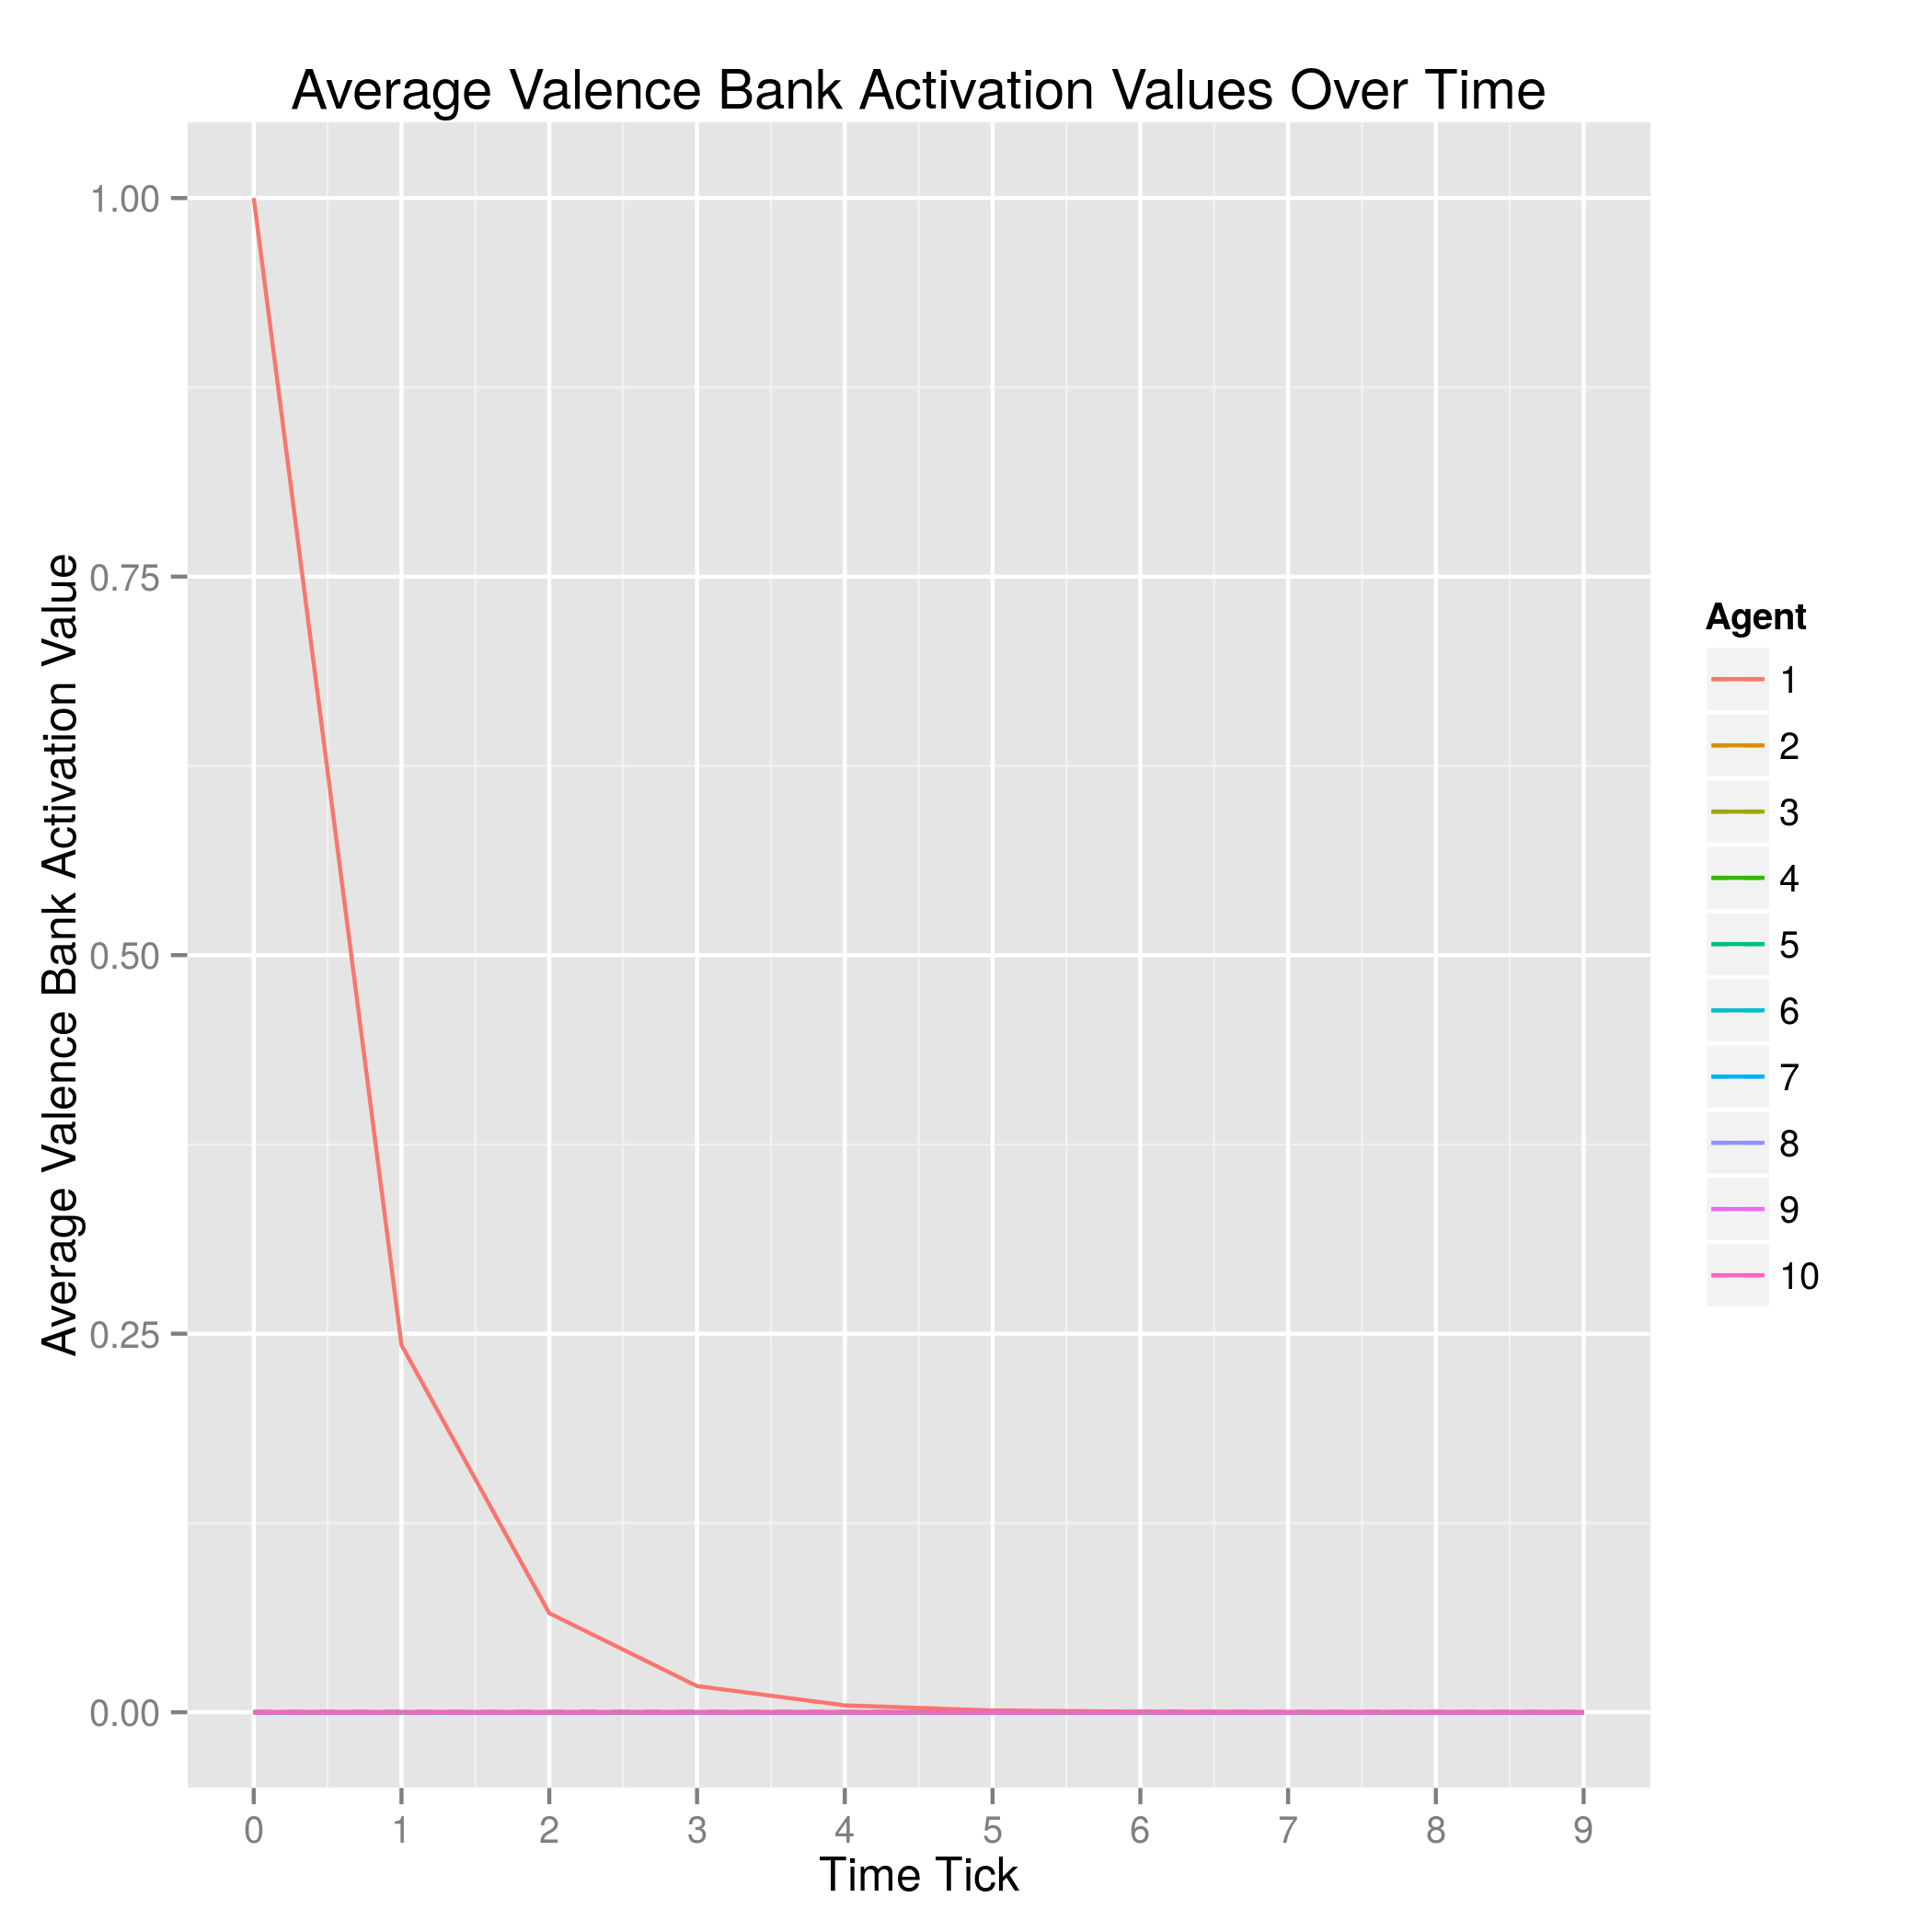
\includegraphics[width=\maxwidth]{figure/plot-sanity1-v2-nostep} \caption[Sanity 1 with re-implemented edge list, no step]{Sanity 1 with re-implemented edge list, no step\label{fig:plot-sanity1-v2-nostep}}
\end{figure}


\end{knitrout}


\newpage
\subsection{Sanity Check 2}
\label{sec:sanity2}
Sanity Case:
\begin{itemize}
  \item Agents Activated: Agent 1 ont
  \item Valence Bank: positive only
  \begin{itemize}
      \item Valence bank activation: \textbf{random}
  \end{itemize}
  \item Valence bank Weights: random
  \begin{itemize}
      \item opposite 0
      \item corresponding 0
      \item carry over = 0.2
      \item bias = 0
      \item decay = -0.5
  \end{itemize}
  \item Network: circle
\end{itemize}

\newpage
\begin{knitrout}
\definecolor{shadecolor}{rgb}{0.969, 0.969, 0.969}\color{fgcolor}\begin{kframe}
\begin{alltt}
\hlkwd{plot.thesis.data}\hlstd{(}\hlstr{"../data/sanity/sanity2-new-external-no-step.csv"}\hlstd{,} \hlkwc{numAgents} \hlstd{=} \hlnum{10}\hlstd{,}
    \hlkwc{numTimeTicks} \hlstd{=} \hlnum{10}\hlstd{)}
\end{alltt}
\end{kframe}\begin{figure}[]

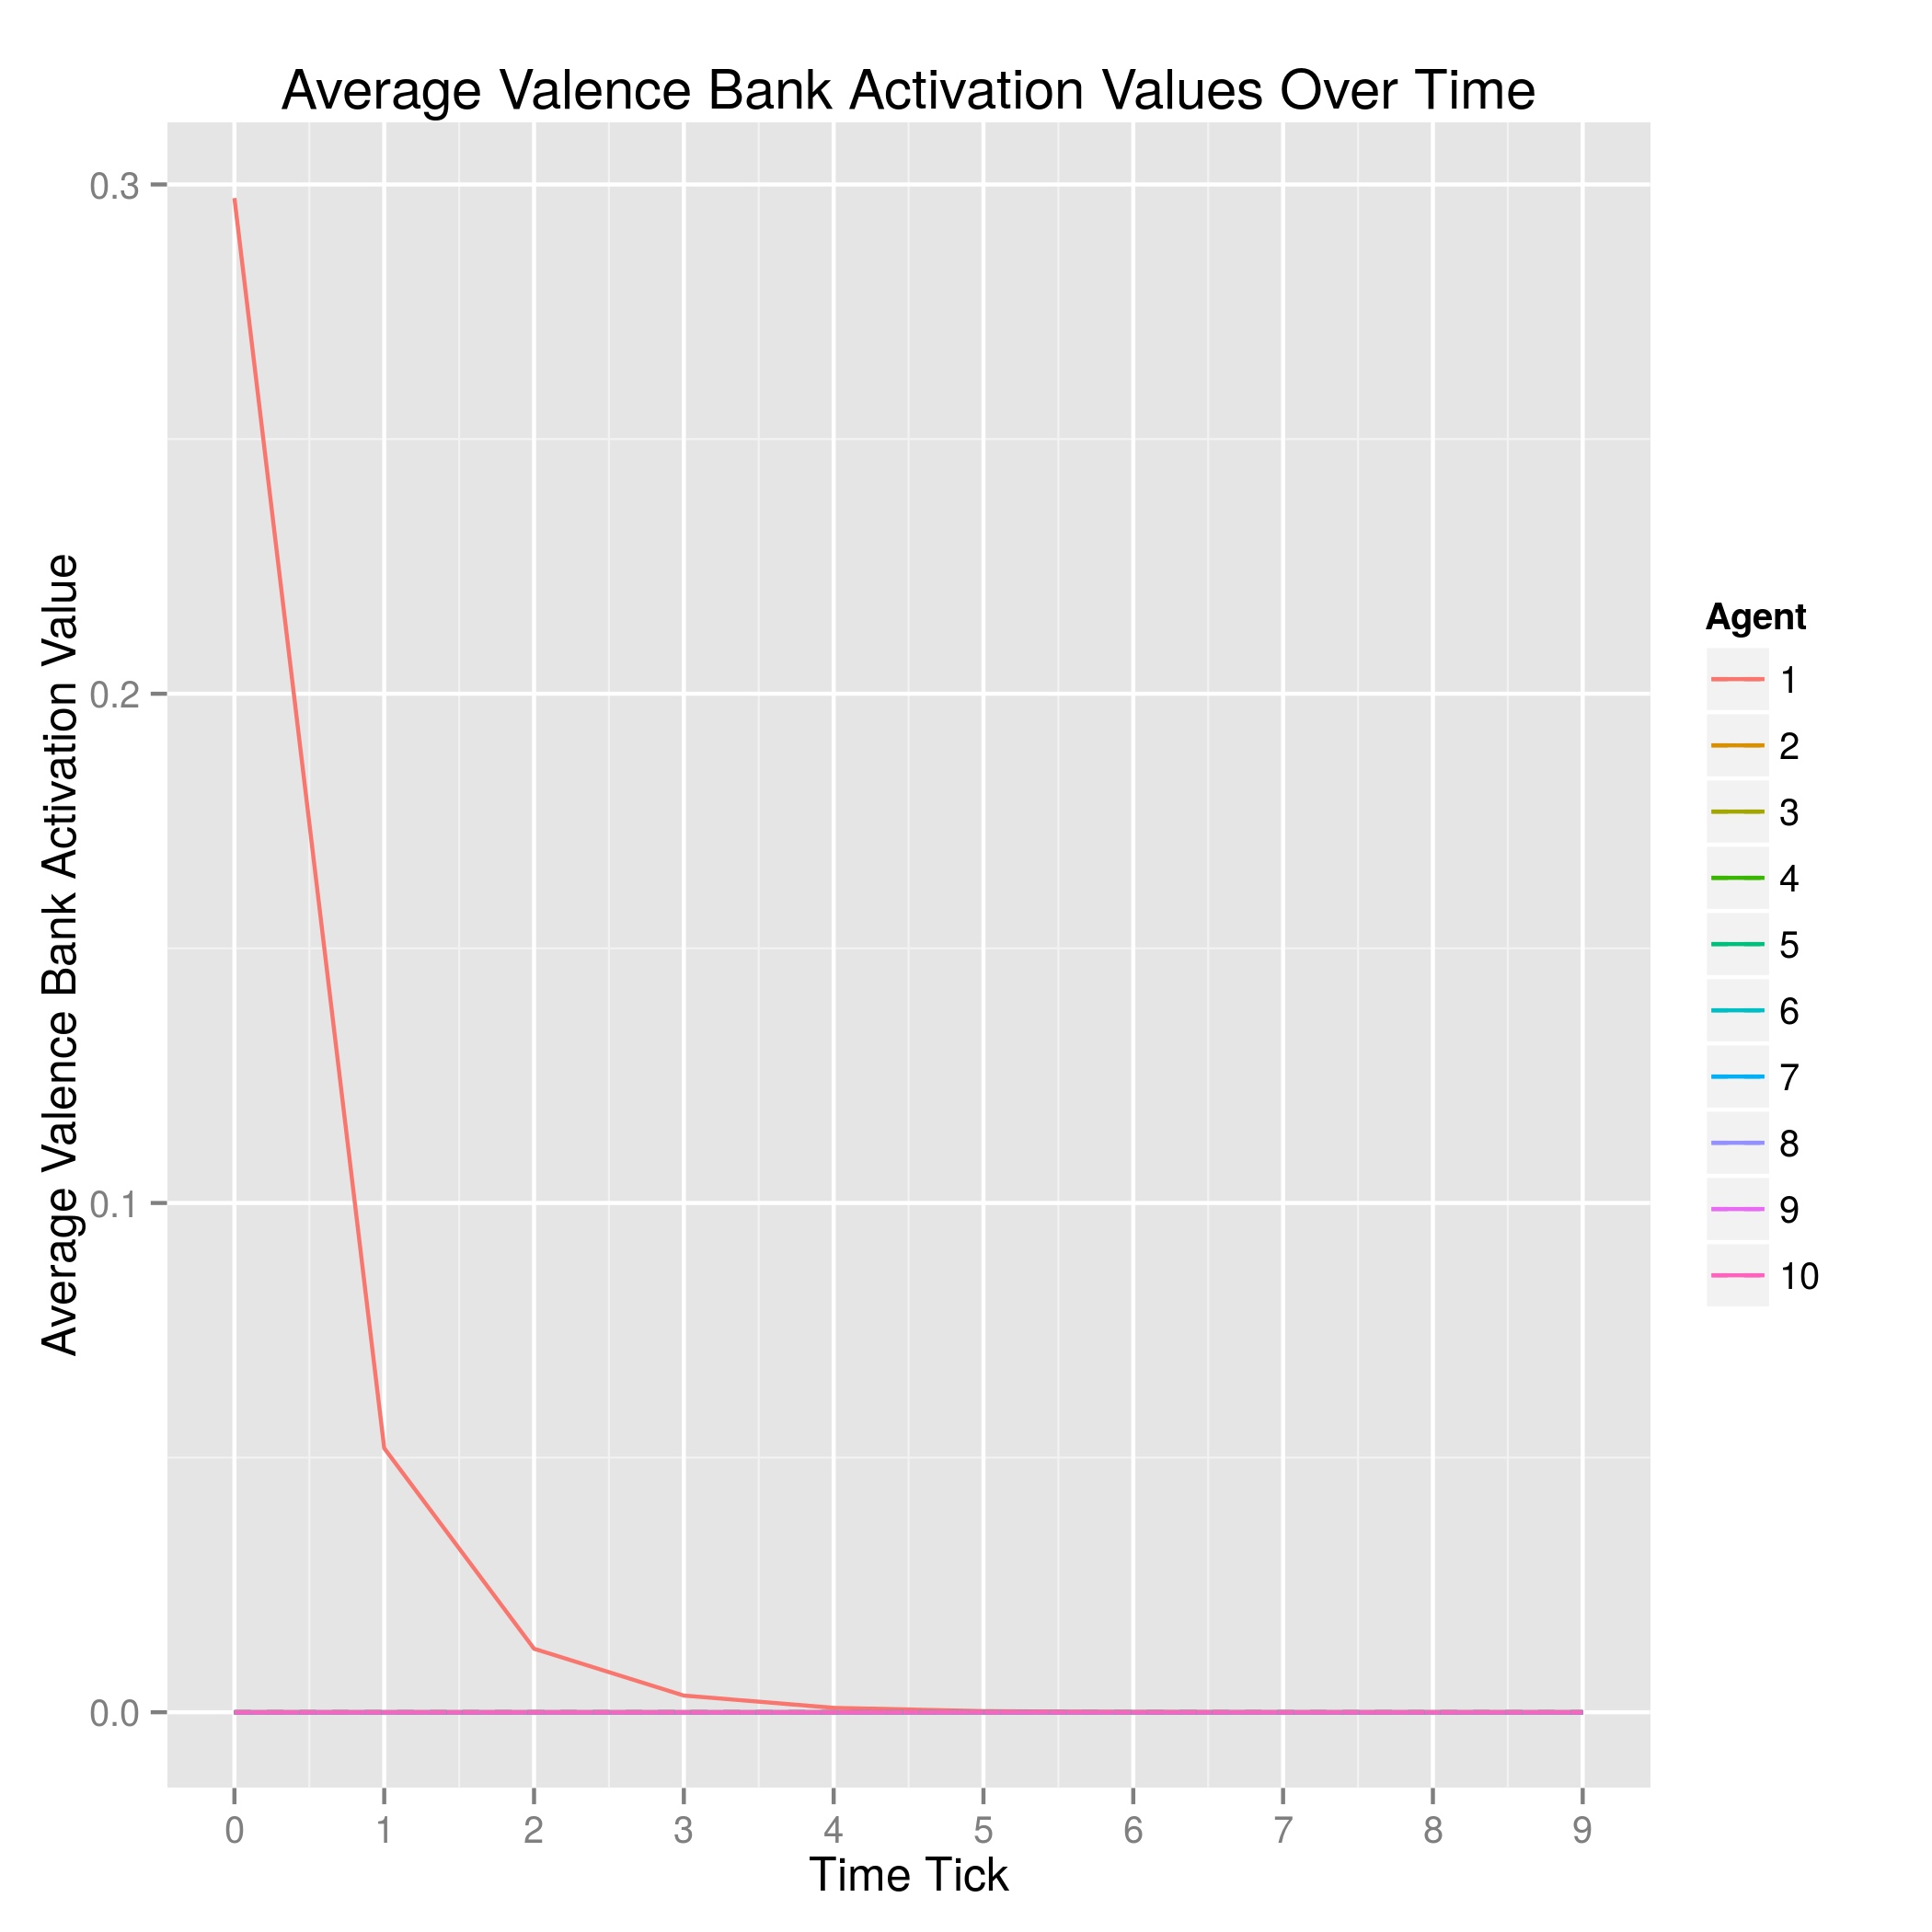
\includegraphics[width=\maxwidth]{figure/plot-sanity-2-v2-nostep} \caption[Sanity Checking 2 with re-implemented edge list, no step]{Sanity Checking 2 with re-implemented edge list, no step\label{fig:plot-sanity-2-v2-nostep}}
\end{figure}


\end{knitrout}


\newpage
\subsection{Sanity Check 3}
\label{sec:sanity3}
Sanity Case:
\begin{itemize}
  \item Agents Activated: Agent 1 ont
  \item Valence Bank: \textbf{both}
  \begin{itemize}
      \item Valence bank activation: random
  \end{itemize}
  \item Valence bank Weights: random
  \begin{itemize}
      \item opposite 0
      \item corresponding 0
      \item carry over = 0.2
      \item bias = 0
      \item decay = -0.5
  \end{itemize}
  \item Network: circle
\end{itemize}

\newpage
\begin{knitrout}
\definecolor{shadecolor}{rgb}{0.969, 0.969, 0.969}\color{fgcolor}\begin{kframe}
\begin{alltt}
\hlkwd{plot.thesis.data}\hlstd{(}\hlstr{"../data/sanity/sanity3-new-external-no-step.csv"}\hlstd{,} \hlkwc{numAgents} \hlstd{=} \hlnum{10}\hlstd{,}
    \hlkwc{numTimeTicks} \hlstd{=} \hlnum{10}\hlstd{)}
\end{alltt}
\end{kframe}\begin{figure}[]

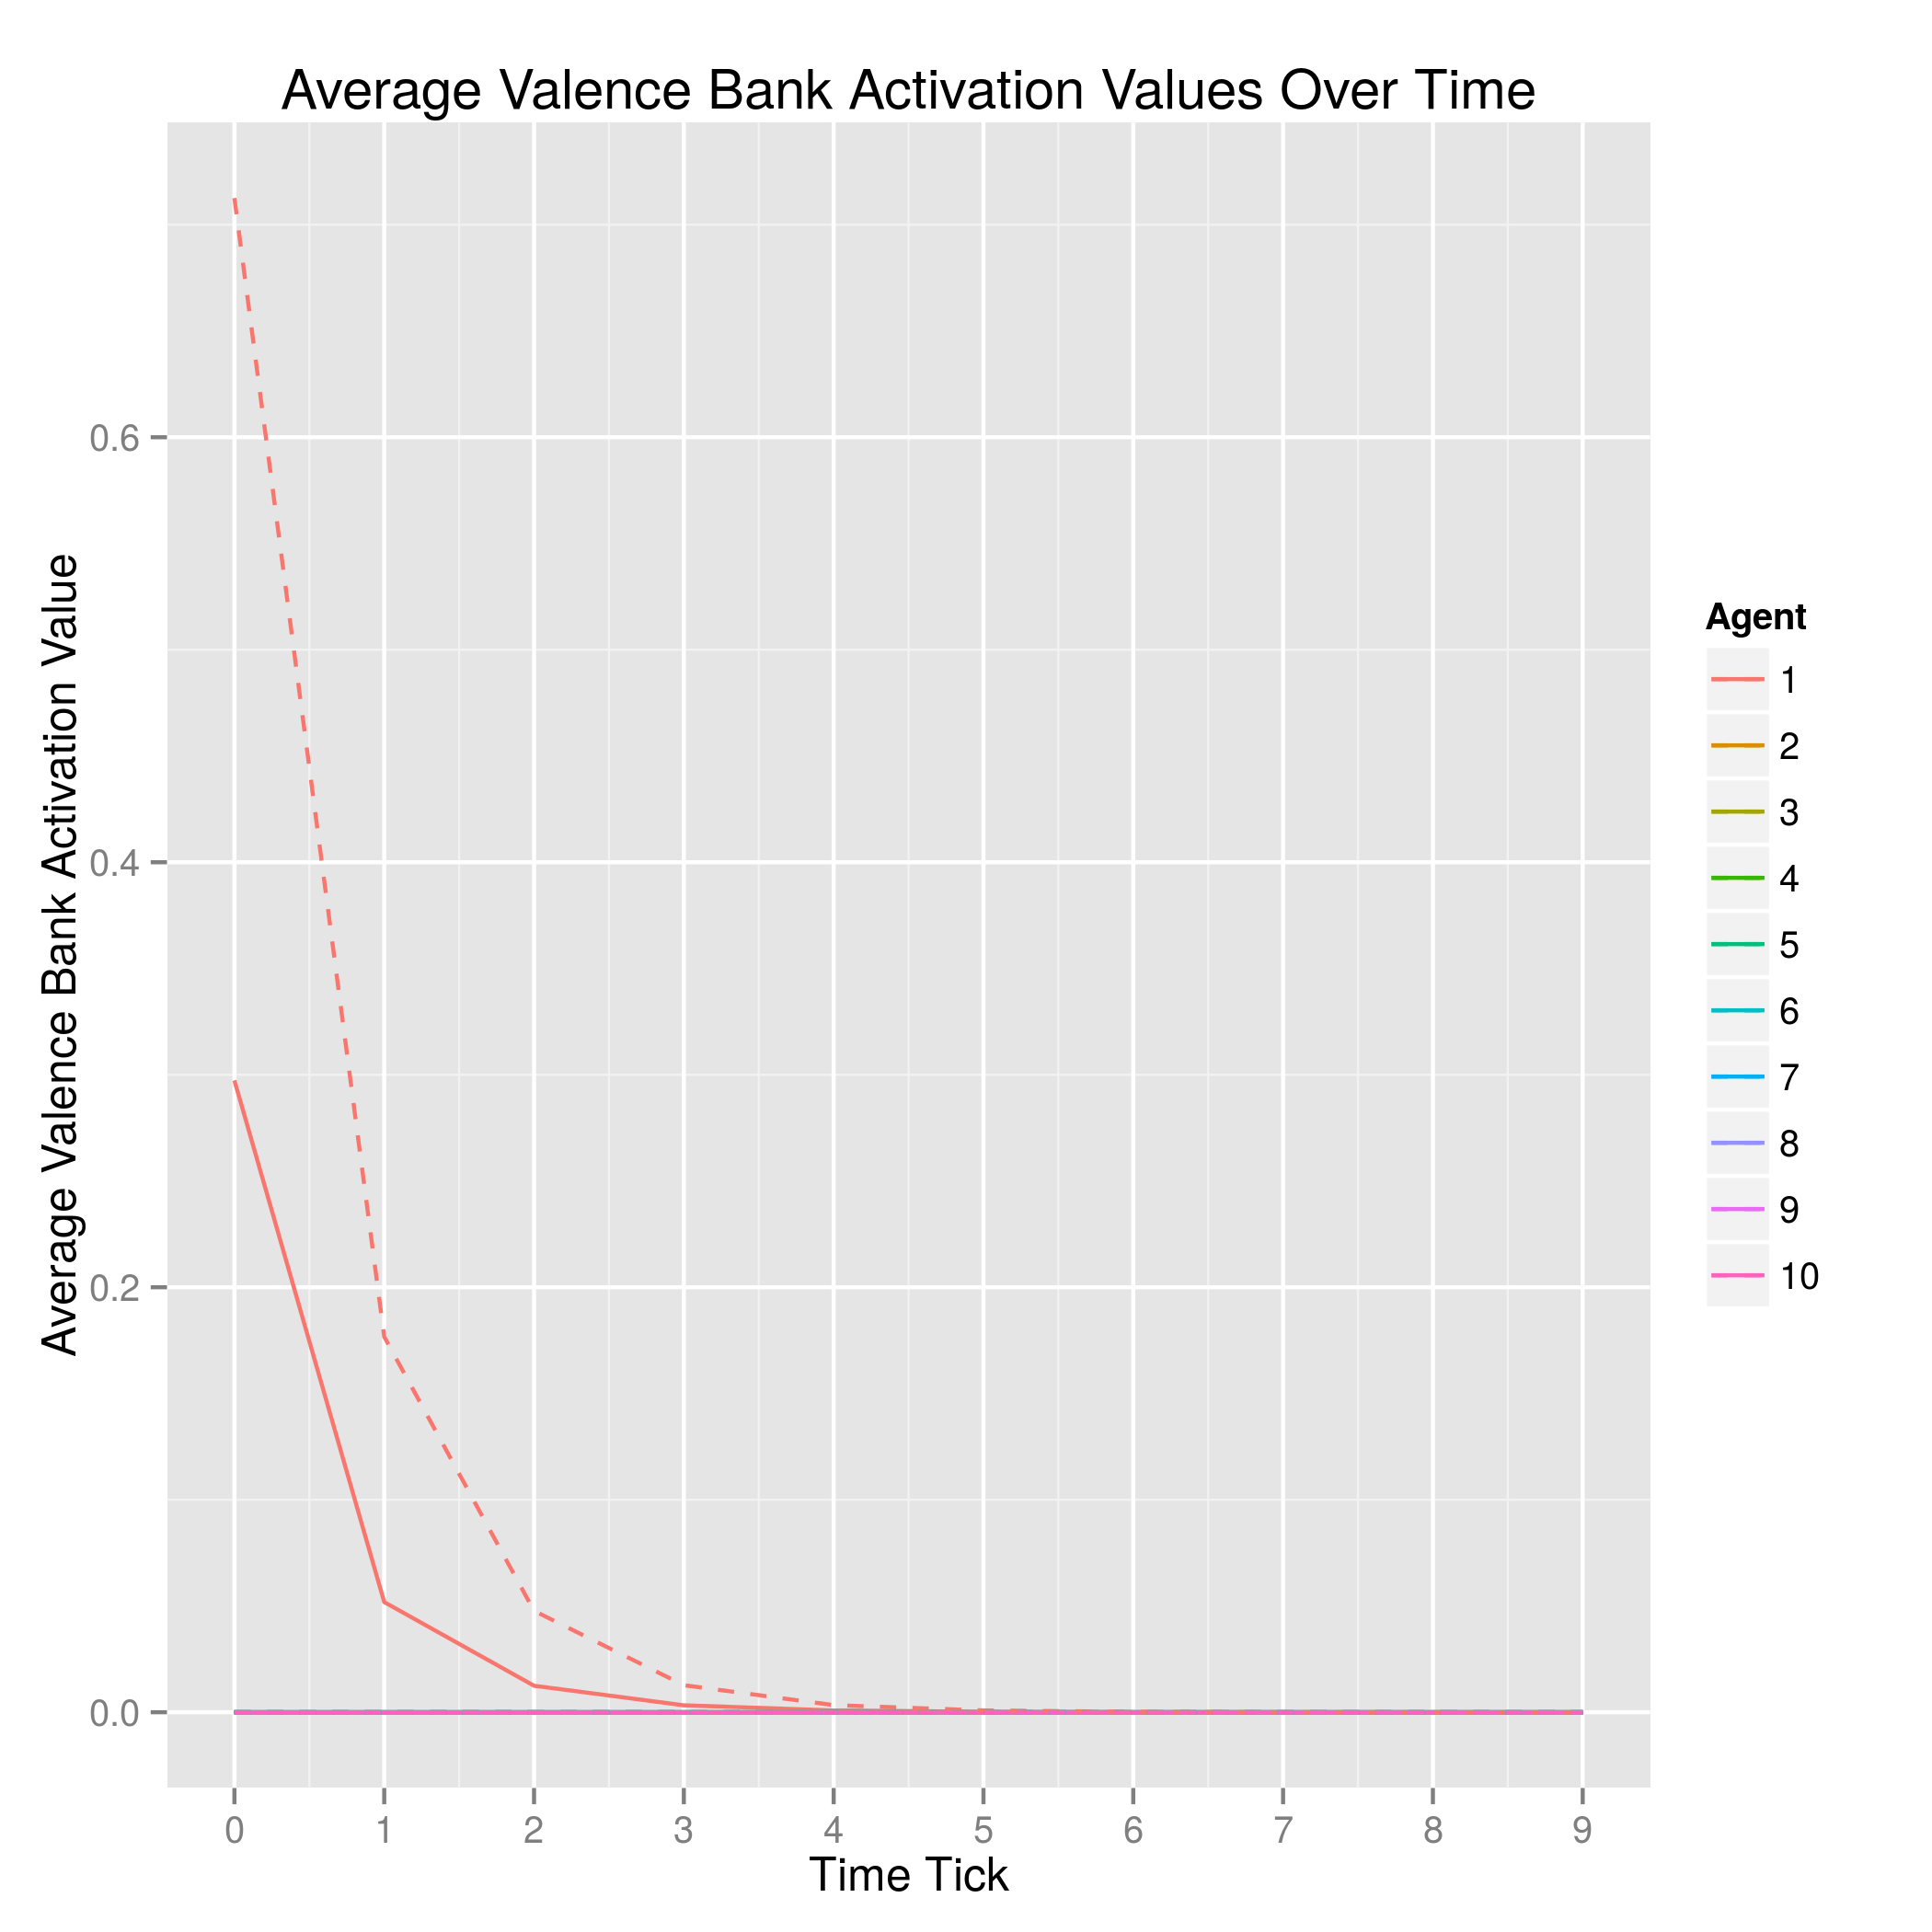
\includegraphics[width=\maxwidth]{figure/plot-sanity-3-v2-nostep} \caption[Sanity Checking 3 with re-implemented edge list, no step]{Sanity Checking 3 with re-implemented edge list, no step\label{fig:plot-sanity-3-v2-nostep}}
\end{figure}


\end{knitrout}


\newpage
\subsection{Sanity Check 4}
\label{sec:sanity4}
Sanity Case:
\begin{itemize}
  \item Agents Activated: Agent 1 ont
  \item Valence Bank: both
  \begin{itemize}
      \item Valence bank activation: random
  \end{itemize}
  \item Valence bank Weights: random
  \begin{itemize}
      \item opposite \textbf{-0.2}
      \item corresponding \textbf{0.5}
      \item carry over = 0.2
      \item bias = 0
      \item decay = -0.5
  \end{itemize}
  \item Network: circle
\end{itemize}

\newpage
\begin{knitrout}
\definecolor{shadecolor}{rgb}{0.969, 0.969, 0.969}\color{fgcolor}\begin{kframe}
\begin{alltt}
\hlkwd{plot.thesis.data}\hlstd{(}\hlstr{"../data/sanity/sanity4-new-external-no-step.csv"}\hlstd{,} \hlkwc{numAgents} \hlstd{=} \hlnum{10}\hlstd{,}
    \hlkwc{numTimeTicks} \hlstd{=} \hlnum{10}\hlstd{)}
\end{alltt}
\end{kframe}\begin{figure}[]

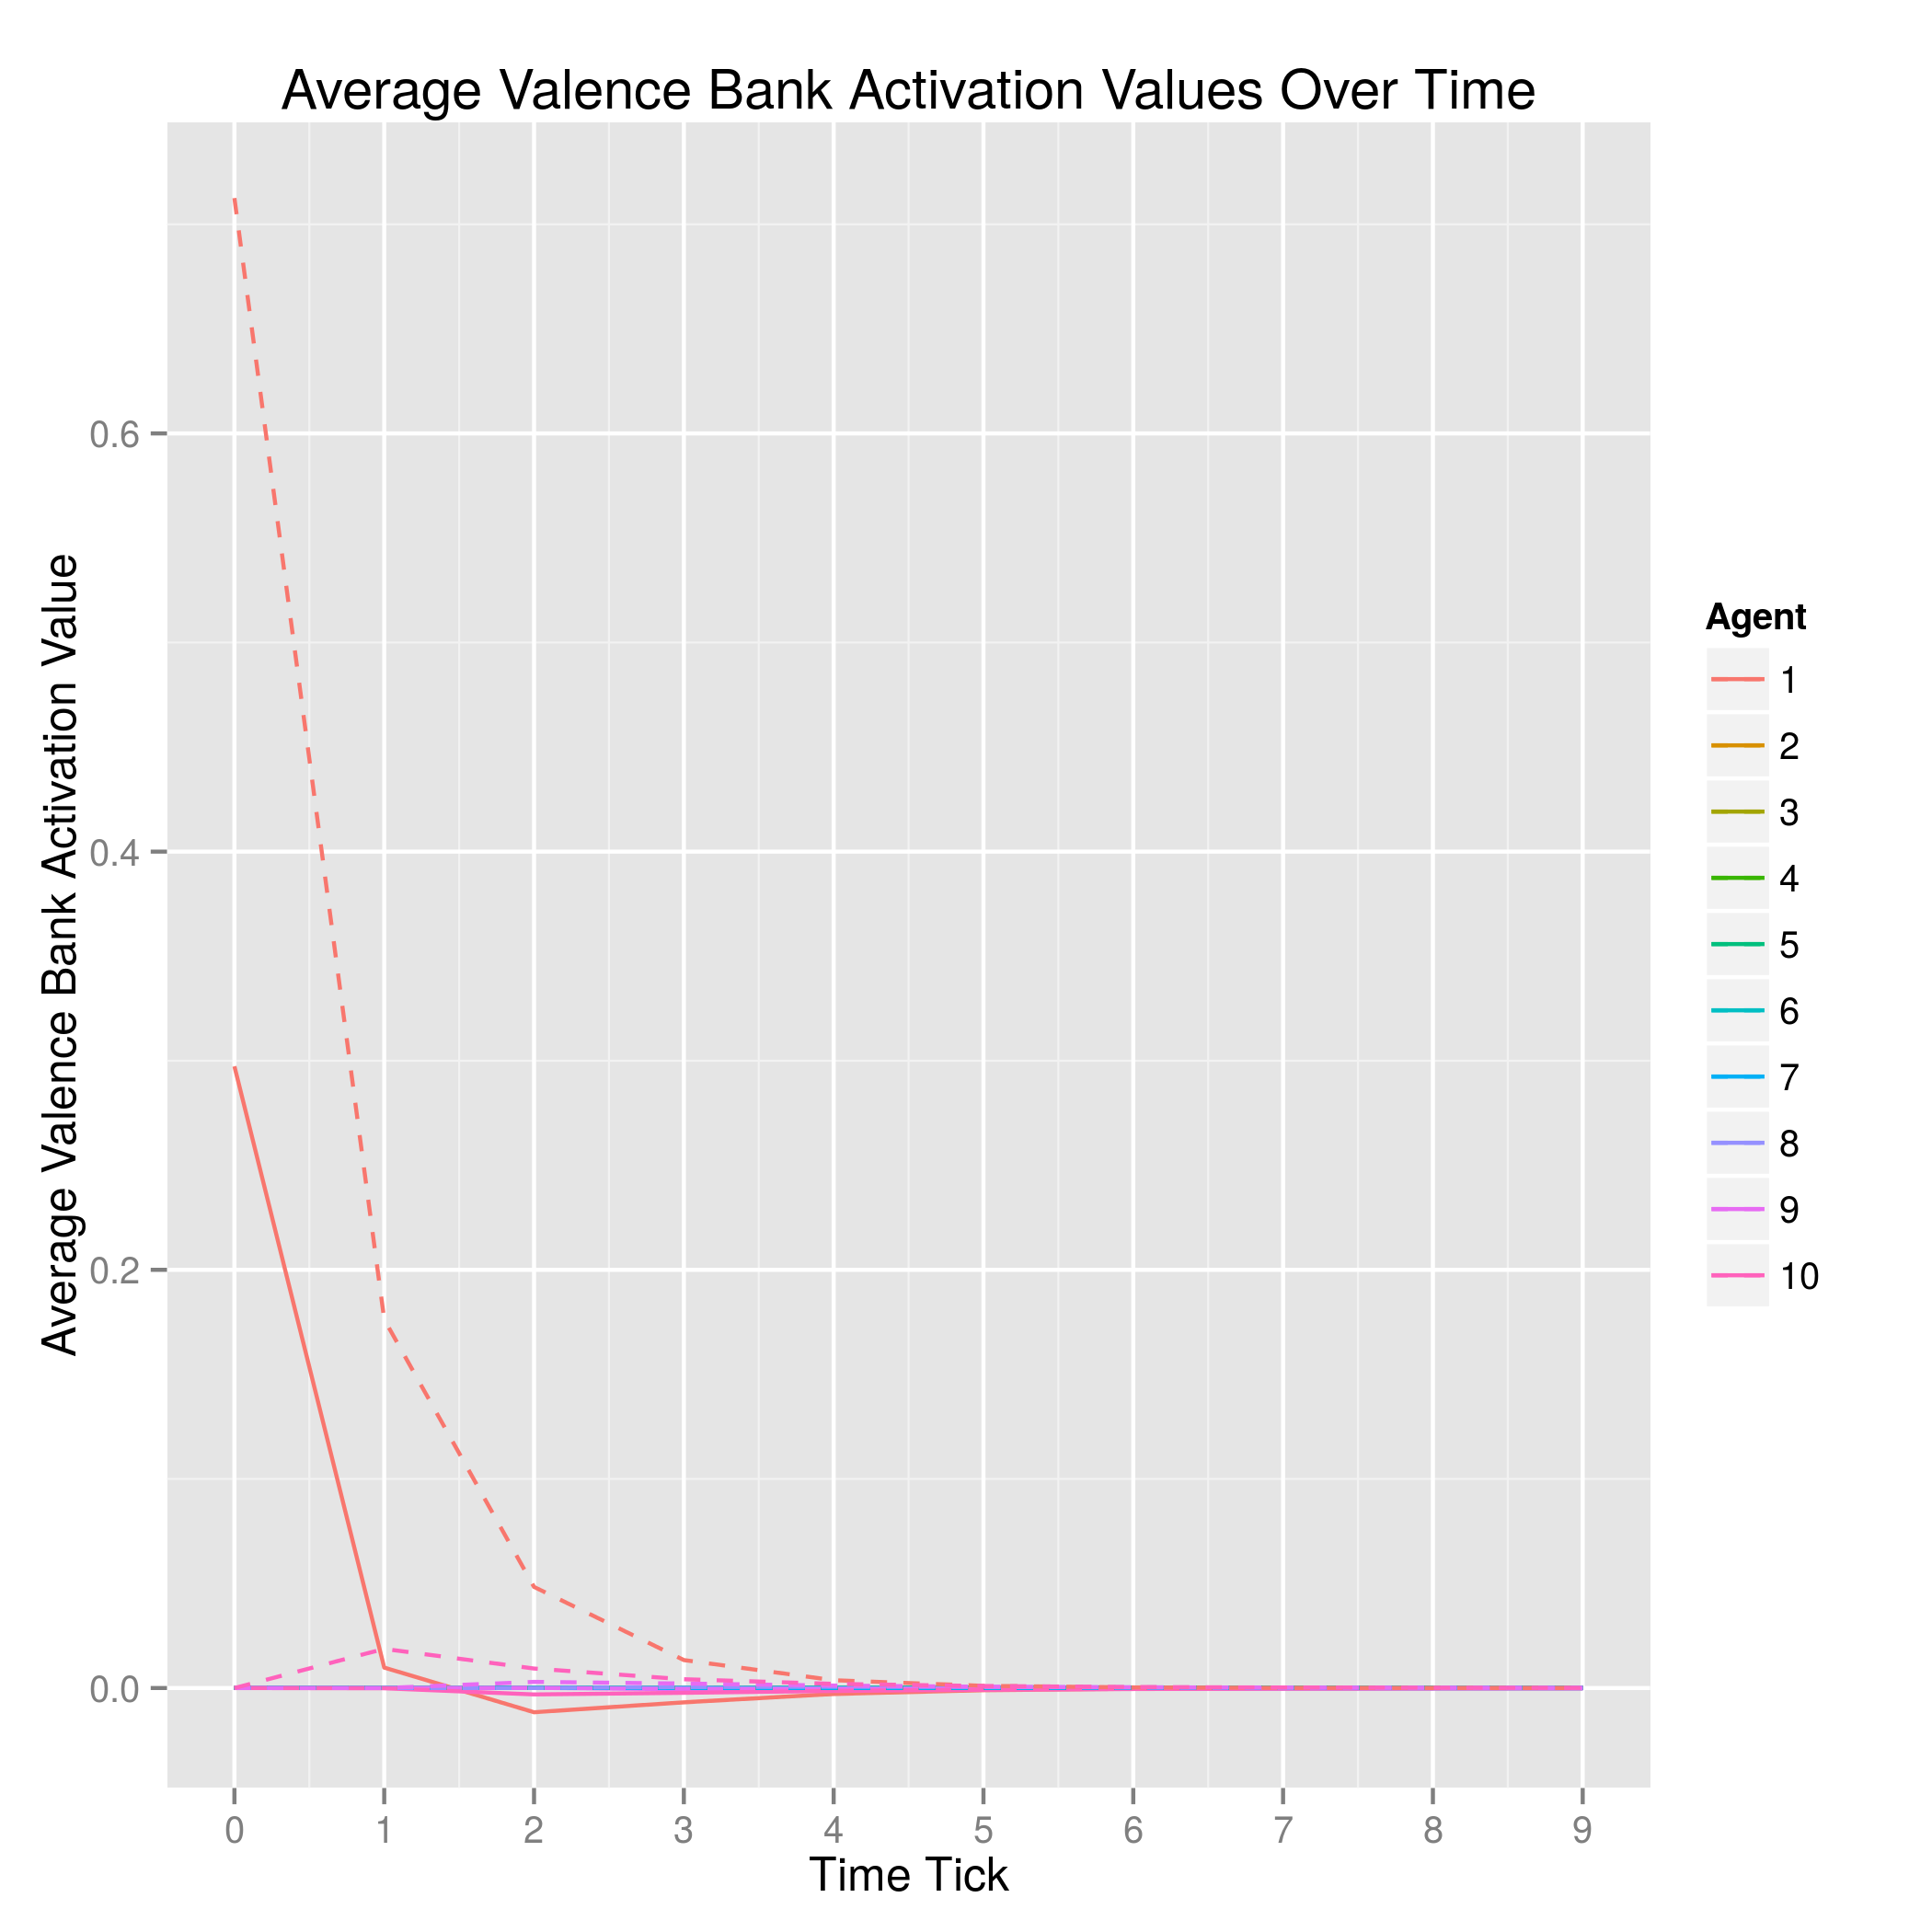
\includegraphics[width=\maxwidth]{figure/plot-sanity-4-v2-nostep} \caption[Sanity Checking 4 with re-implemented edge list, no step]{Sanity Checking 4 with re-implemented edge list, no step\label{fig:plot-sanity-4-v2-nostep}}
\end{figure}


\end{knitrout}


\newpage
\subsection{Sanity Check 5}
\label{sec:sanity5}
Sanity Case:
\begin{itemize}
  \item Agents Activated: \textbf{All}
  \item Valence Bank: both
  \begin{itemize}
      \item Valence bank activation: random
  \end{itemize}
  \item Valence bank Weights: random
  \begin{itemize}
      \item opposite -0.2
      \item corresponding 0.5
      \item carry over = 0.2
      \item bias = 0
      \item decay = -0.5
  \end{itemize}
  \item Network: circle
\end{itemize}

\newpage
\begin{knitrout}
\definecolor{shadecolor}{rgb}{0.969, 0.969, 0.969}\color{fgcolor}\begin{kframe}
\begin{alltt}
\hlkwd{plot.thesis.data}\hlstd{(}\hlstr{"../data/sanity/sanity5-new-external-no-step.csv"}\hlstd{,} \hlkwc{numAgents} \hlstd{=} \hlnum{10}\hlstd{,}
    \hlkwc{numTimeTicks} \hlstd{=} \hlnum{10}\hlstd{)}
\end{alltt}
\end{kframe}\begin{figure}[]

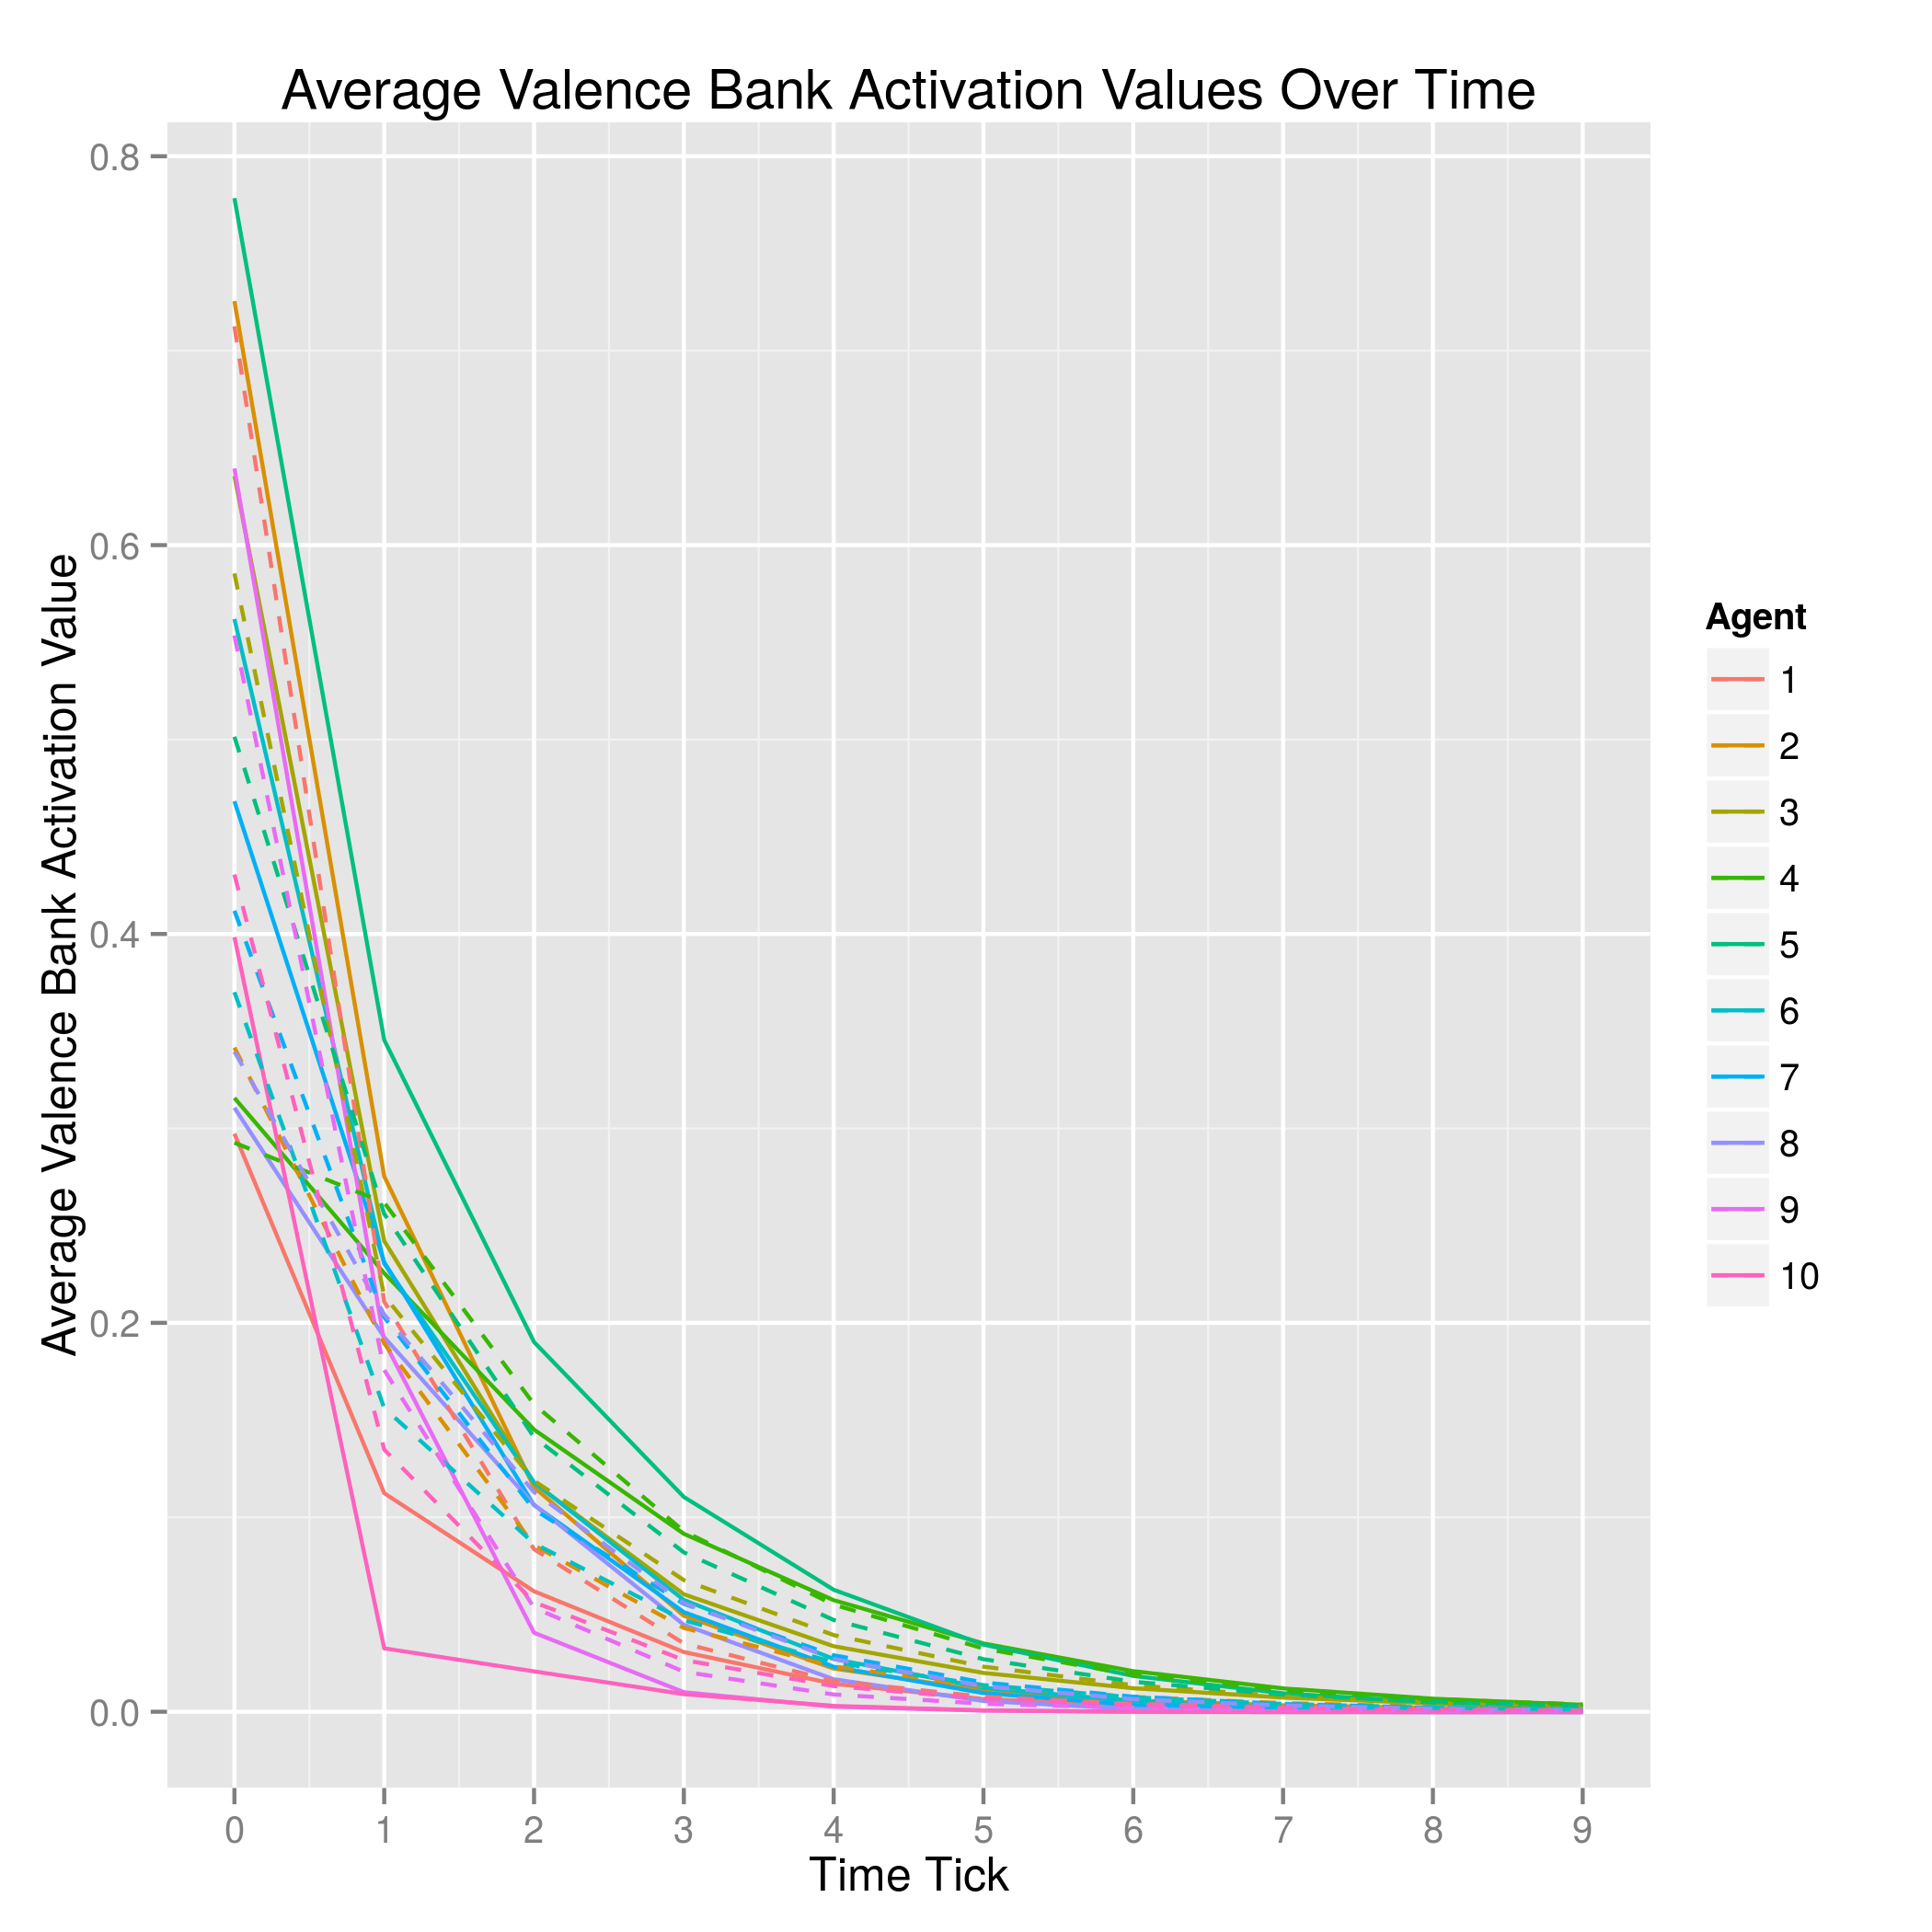
\includegraphics[width=\maxwidth]{figure/plot-sanity-5-v2-nostep} \caption[Sanity Checking 5 with re-implemented edge list, no step]{Sanity Checking 5 with re-implemented edge list, no step\label{fig:plot-sanity-5-v2-nostep}}
\end{figure}


\end{knitrout}


\newpage
\subsection{Sanity 6}
\label{sec:sanity6}
Sanity Case:
\begin{itemize}
  \item Agents Activated: All
  \item Valence Bank: both
  \begin{itemize}
      \item Valence bank activation: random
  \end{itemize}
  \item Valence bank Weights: random
  \begin{itemize}
      \item opposite -0.2
      \item corresponding 0.5
      \item carry over = 0.2
      \item bias = 0
      \item decay = -0.5
  \end{itemize}
  \item Network: \textbf{circle network, however agent 5 has no inputs, and multiple agents influence agent 1}
\end{itemize}
\begin{knitrout}
\definecolor{shadecolor}{rgb}{0.969, 0.969, 0.969}\color{fgcolor}\begin{kframe}
\begin{alltt}
\hlkwd{plot.thesis.data}\hlstd{(}\hlstr{"../data/sanity/sanity6.csv"}\hlstd{,} \hlkwc{numAgents} \hlstd{=} \hlnum{10}\hlstd{,} \hlkwc{numTimeTicks} \hlstd{=} \hlnum{10}\hlstd{)}
\end{alltt}
\end{kframe}\begin{figure}[]

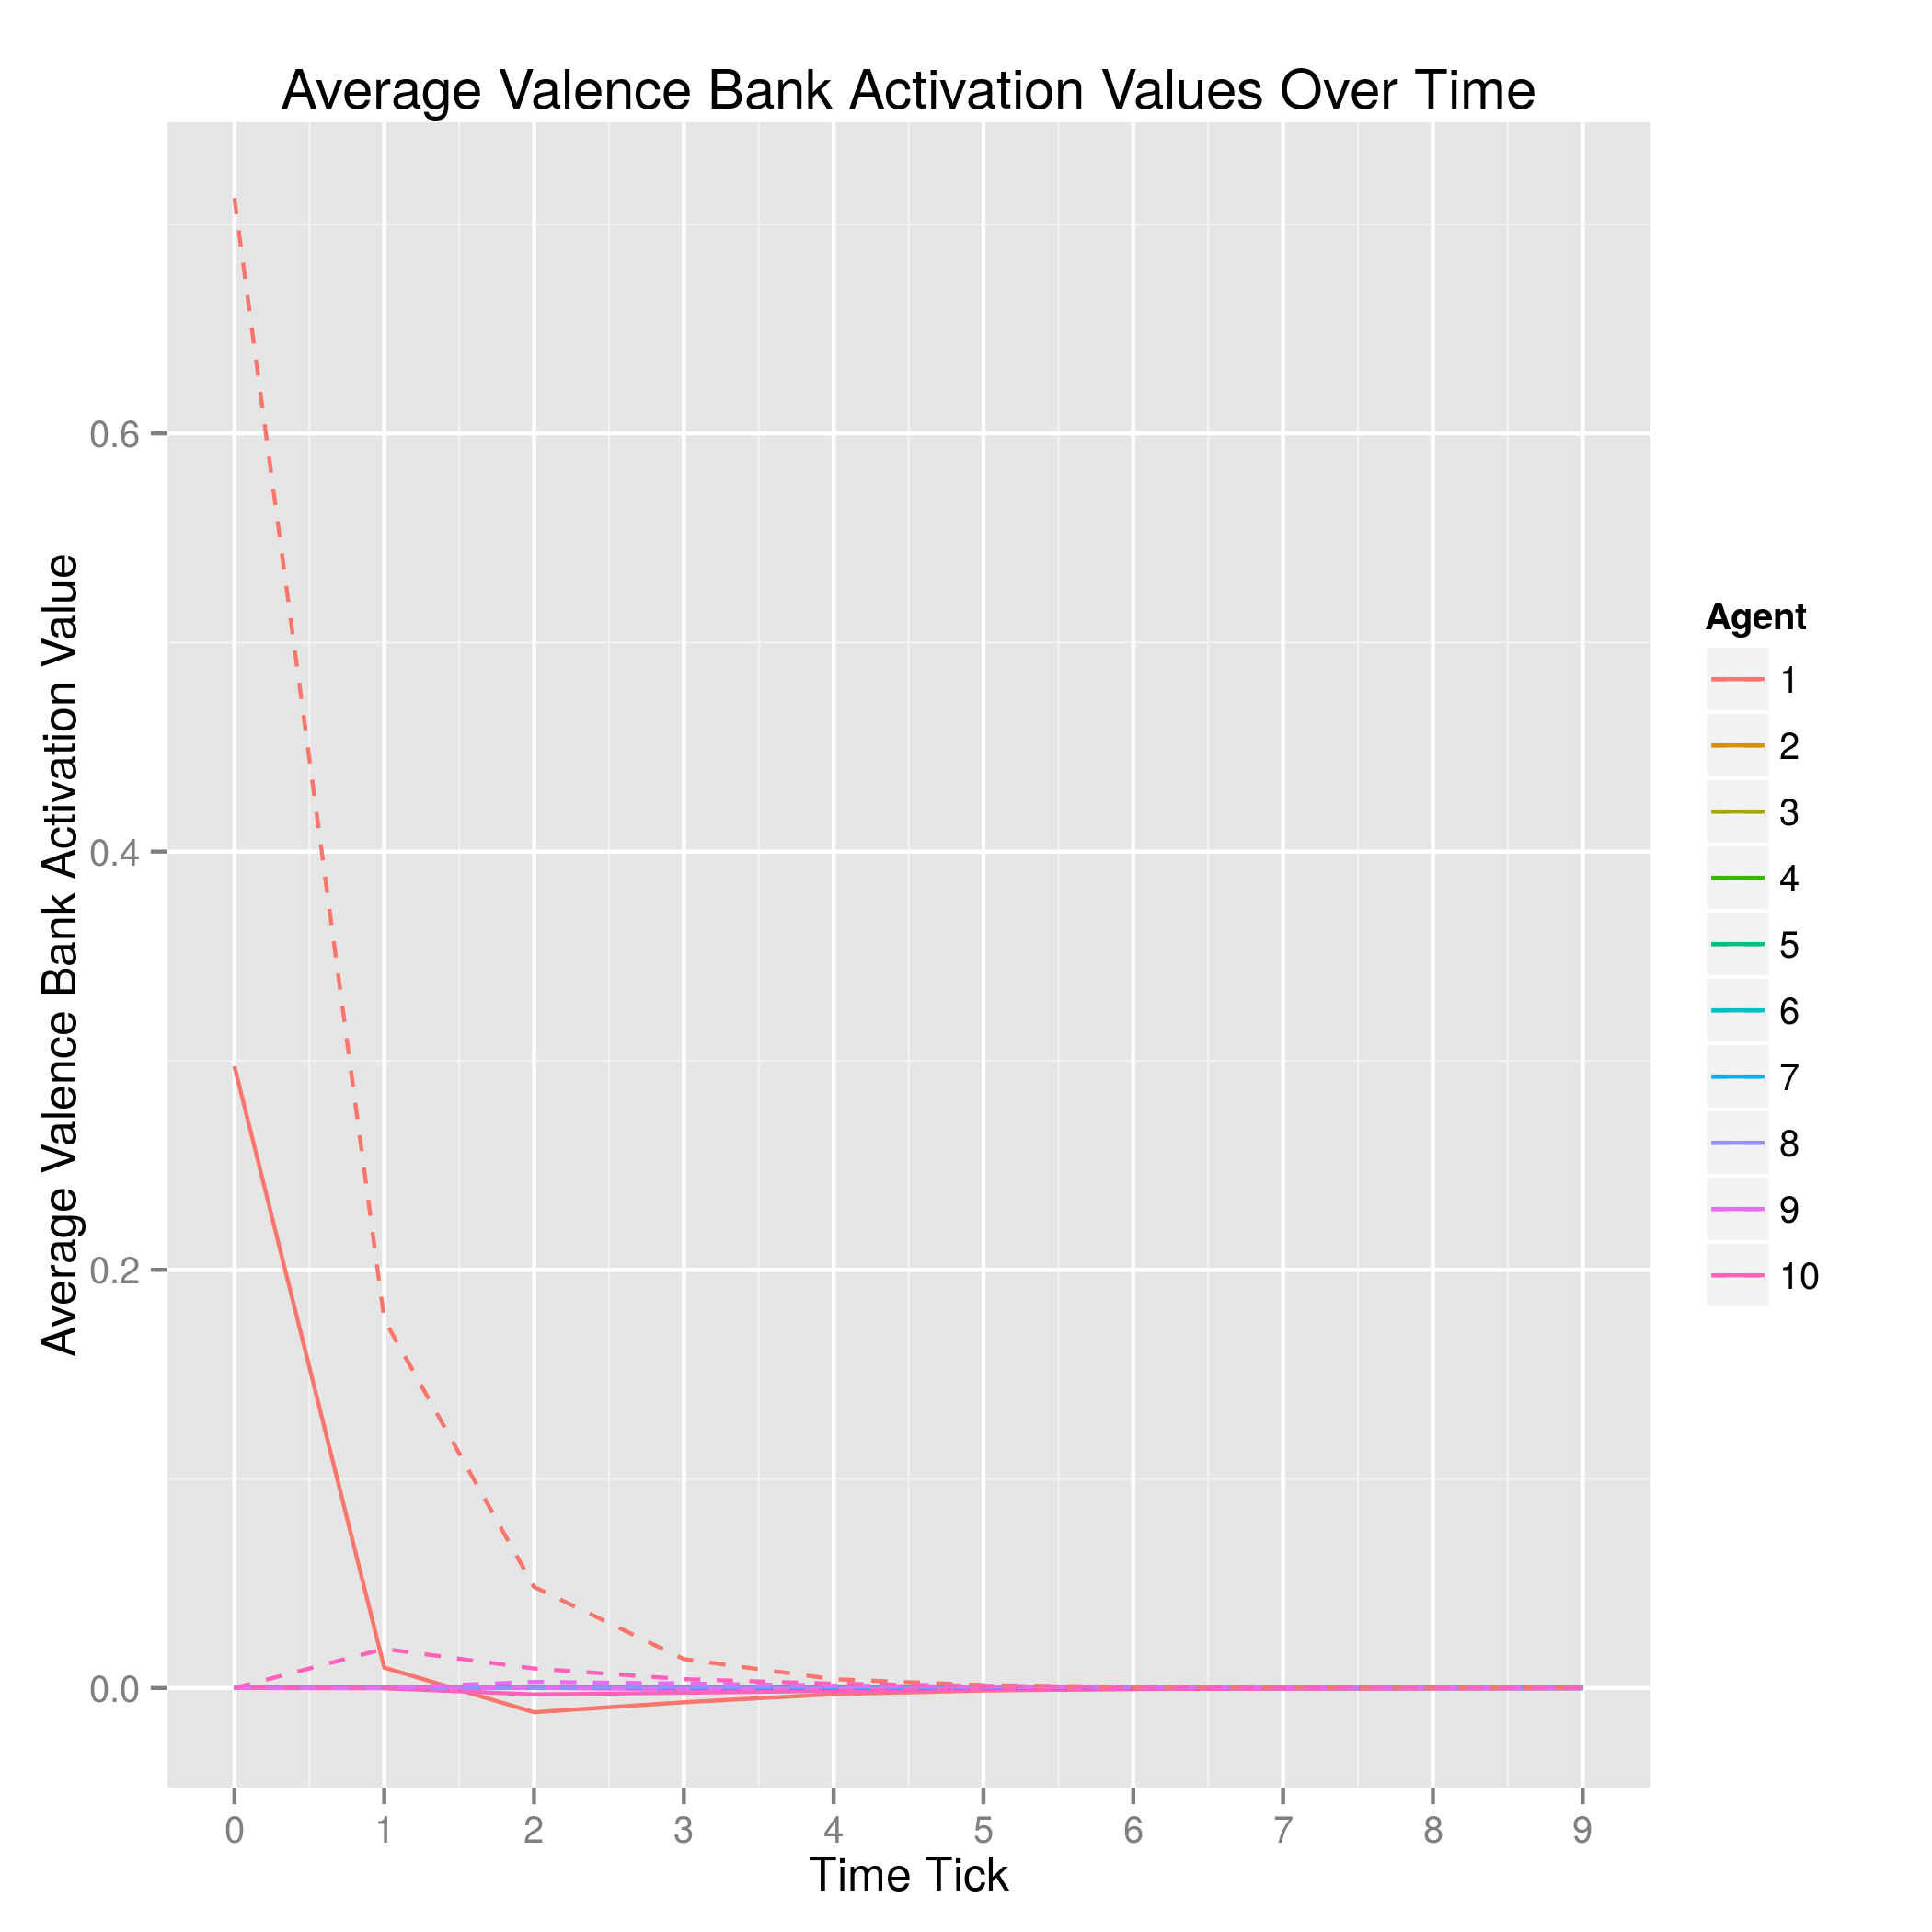
\includegraphics[width=\maxwidth]{figure/plot-sanity-6} \caption[Sanity Checking 6 with re-implemented edge list]{Sanity Checking 6 with re-implemented edge list\label{fig:plot-sanity-6}}
\end{figure}


\end{knitrout}


\newpage
\subsubsection{Sanity 6 no decay}
\label{sec:sanity6-nodecay}
\begin{knitrout}
\definecolor{shadecolor}{rgb}{0.969, 0.969, 0.969}\color{fgcolor}\begin{kframe}
\begin{alltt}
\hlkwd{plot.thesis.data}\hlstd{(}\hlstr{"../data/sanity/sanity6-nodecay.csv"}\hlstd{,} \hlkwc{numAgents} \hlstd{=} \hlnum{10}\hlstd{,} \hlkwc{numTimeTicks} \hlstd{=} \hlnum{10}\hlstd{)}
\end{alltt}
\end{kframe}\begin{figure}[]

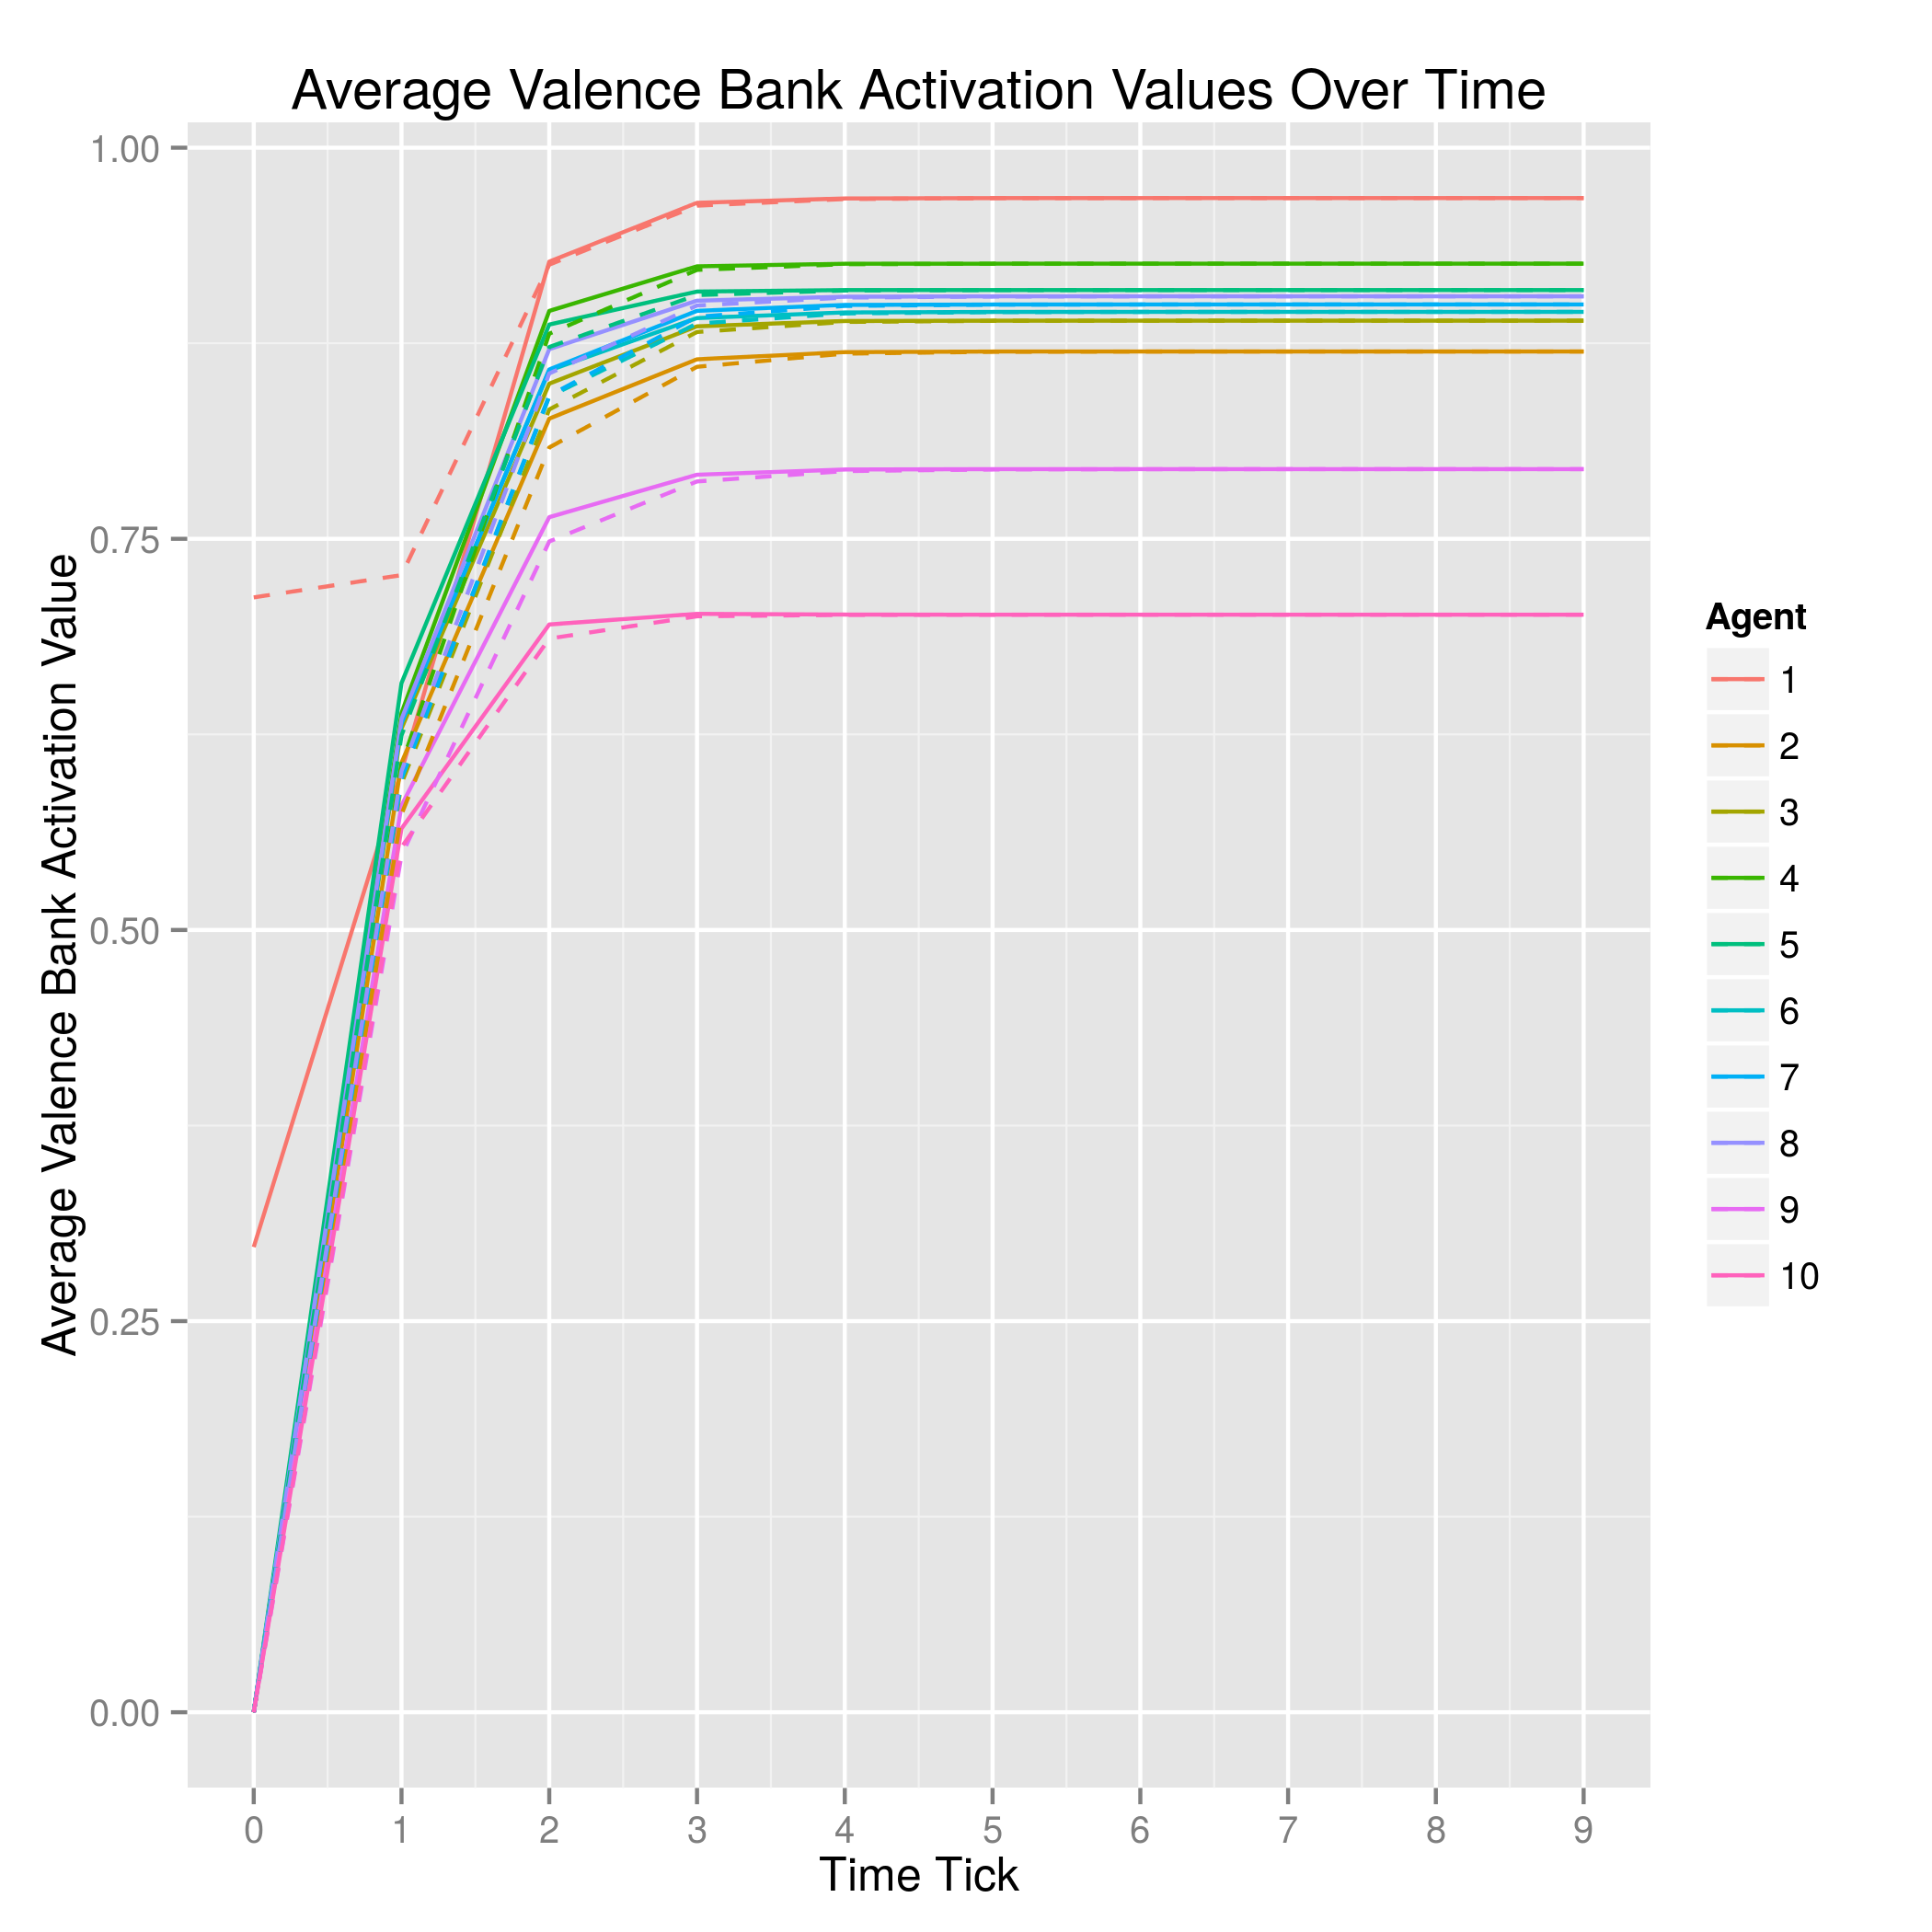
\includegraphics[width=\maxwidth]{figure/plot-sanity-6-nodecay} \caption[Sanity Checking 6 with re-implemented edge list no decay]{Sanity Checking 6 with re-implemented edge list no decay\label{fig:plot-sanity-6-nodecay}}
\end{figure}


\end{knitrout}


\newpage
\subsection{Sanity 7}
\label{sec:sanity7}
Sanity Case:
\begin{itemize}
  \item Agents Activated: All
  \item Valence Bank: both
  \begin{itemize}
      \item Valence bank activation: random
  \end{itemize}
  \item Valence bank Weights: random
  \begin{itemize}
      \item opposite -0.2
      \item corresponding 0.5
      \item carry over = 0.2
      \item bias = 0
      \item decay = -0.5
  \end{itemize}
  \item Network: circle network, however agent 5 has no inputs, and multiple agents influence agent 1
\end{itemize}
\begin{knitrout}
\definecolor{shadecolor}{rgb}{0.969, 0.969, 0.969}\color{fgcolor}\begin{kframe}
\begin{alltt}
\hlkwd{plot.thesis.data}\hlstd{(}\hlstr{"../data/sanity/sanity7-nodecay.csv"}\hlstd{,} \hlkwc{numAgents} \hlstd{=} \hlnum{10}\hlstd{,} \hlkwc{numTimeTicks} \hlstd{=} \hlnum{10}\hlstd{)}
\end{alltt}
\end{kframe}\begin{figure}[]

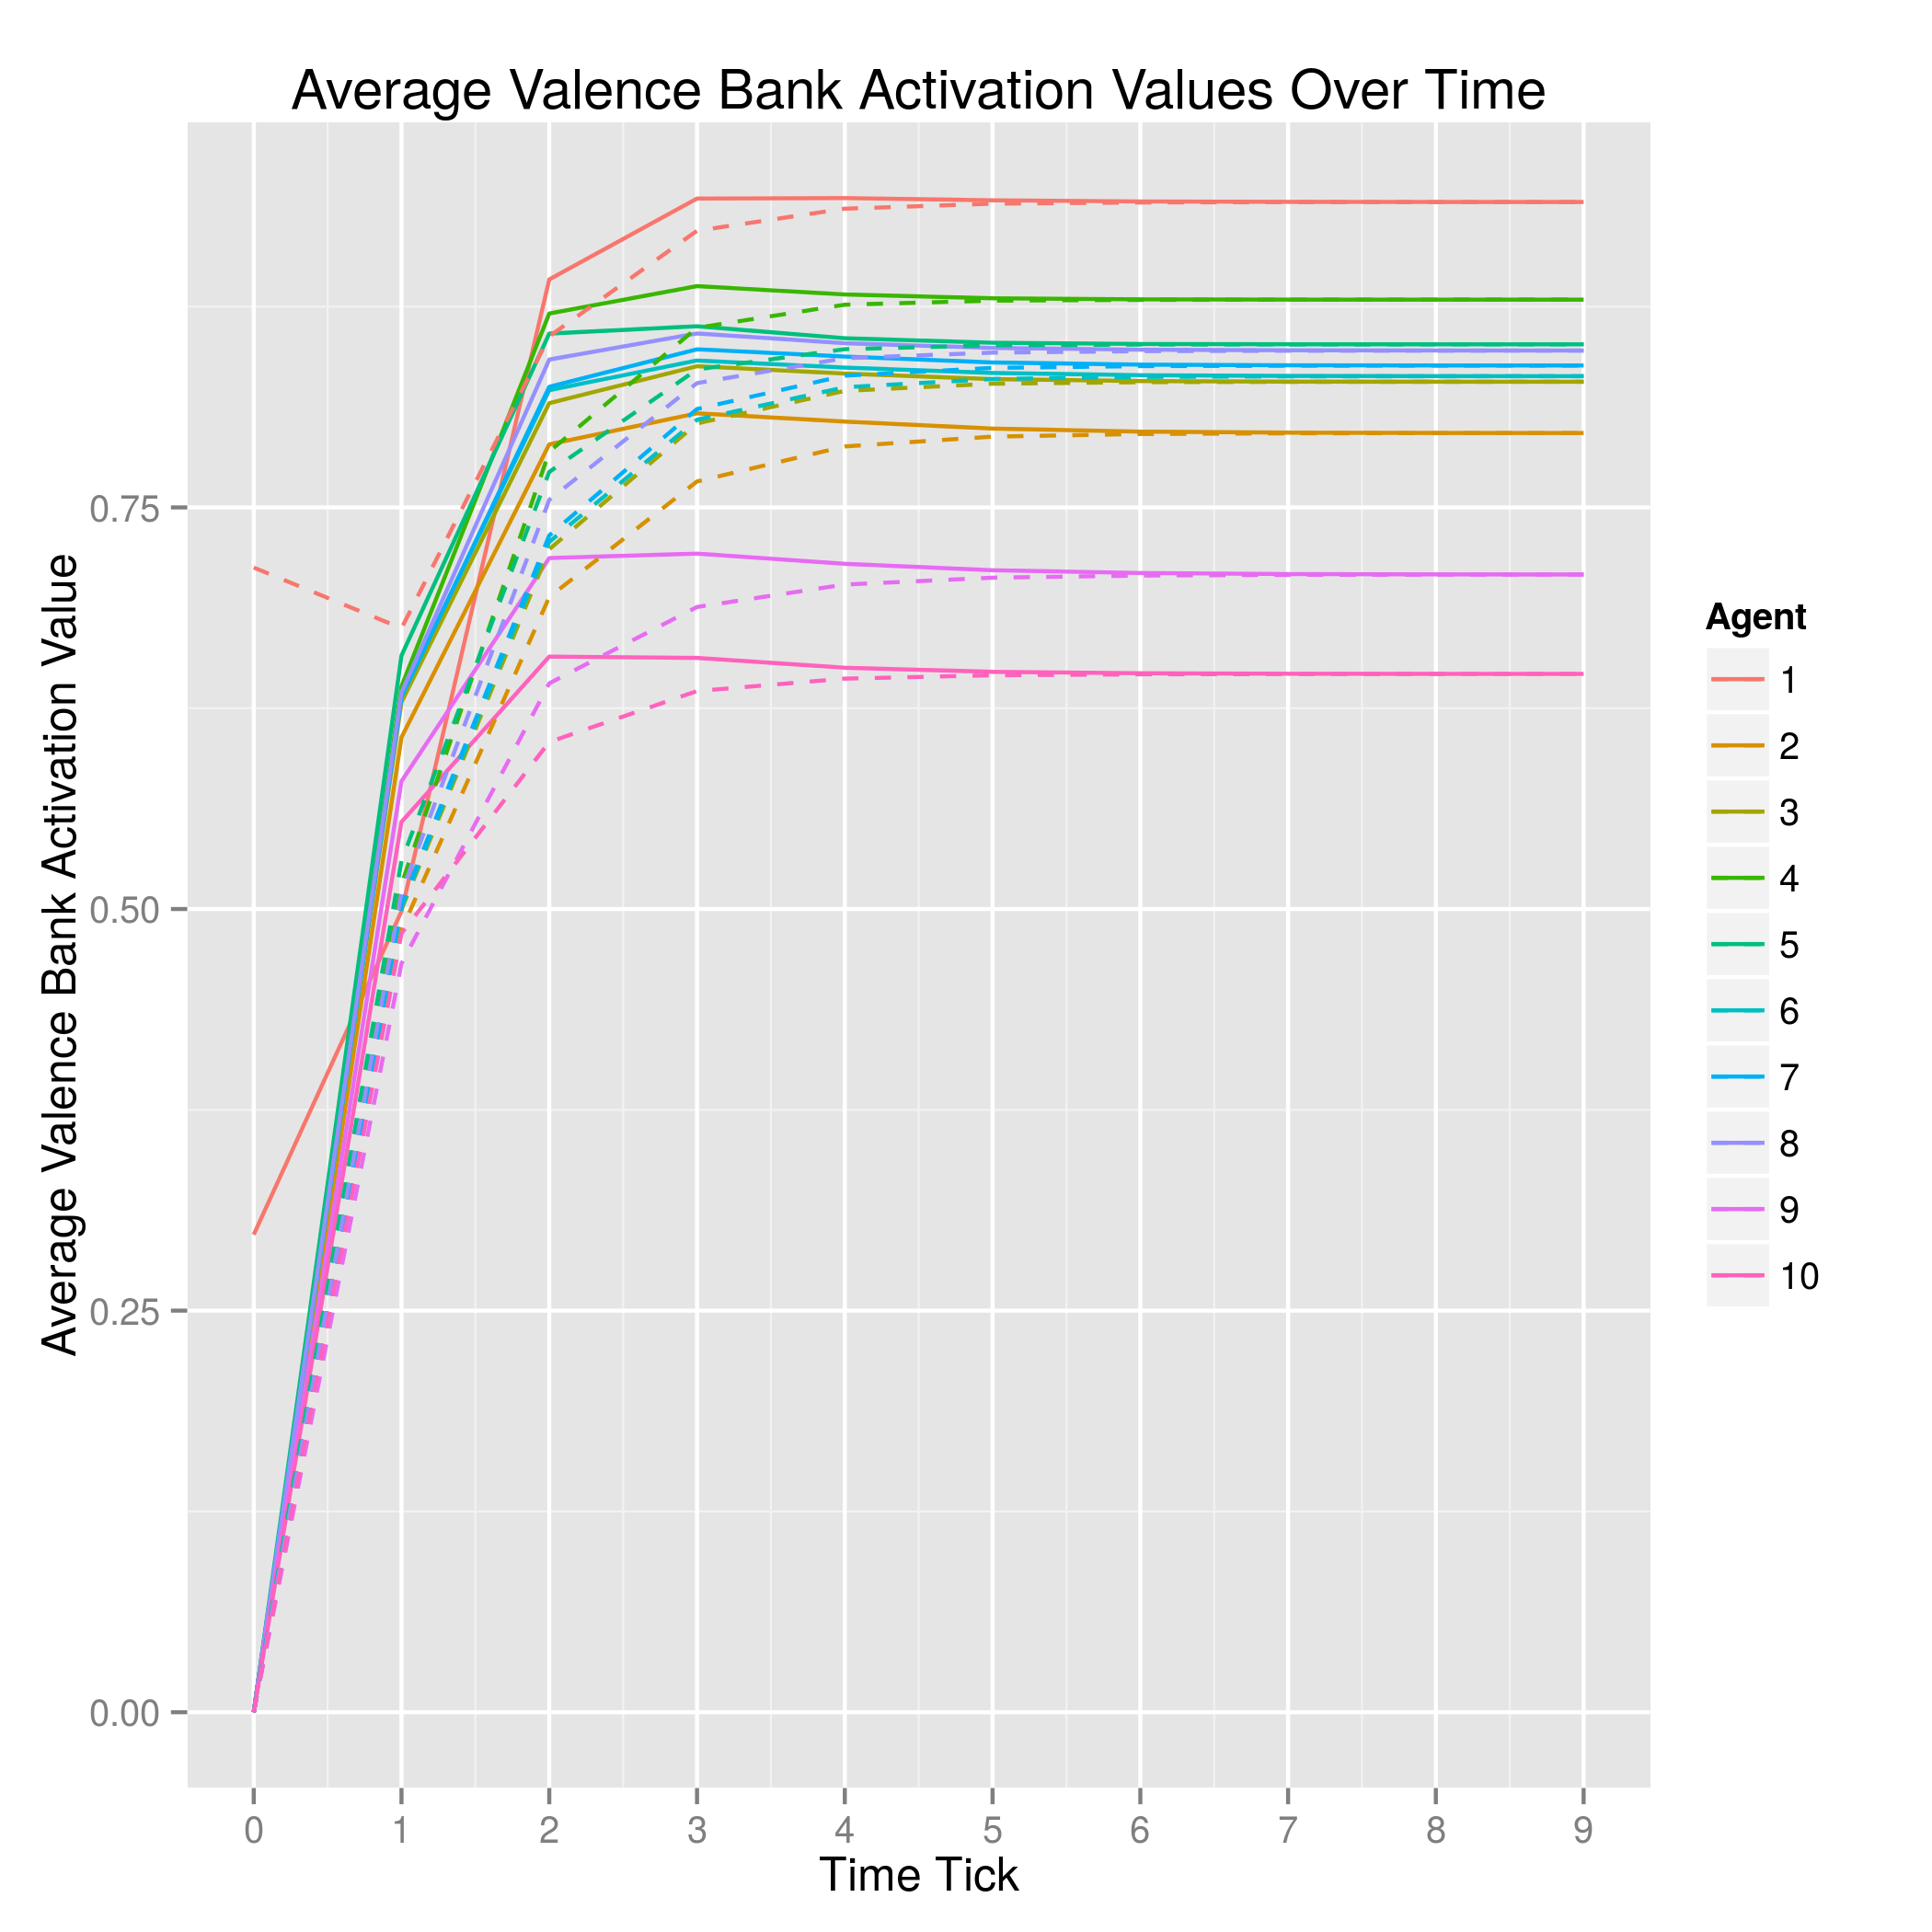
\includegraphics[width=\maxwidth]{figure/plot-sanity-7-nodecay} \caption[Sanity Checking 7 with re-implemented edge list no decay]{Sanity Checking 7 with re-implemented edge list no decay\label{fig:plot-sanity-7-nodecay}}
\end{figure}


\end{knitrout}


\newpage
\subsection{Sanity 8}
\label{sec:sanity8}
\begin{itemize}
  \item Agents Activated: \textbf{1}
  \item Valence Bank: both
  \begin{itemize}
      \item Valence bank activation: \textbf{first positive, last negative}
  \end{itemize}
  \item Valence bank Weights: random
  \begin{itemize}
      \item opposite -0.2
      \item corresponding 0.5
      \item carry over = 0.2
      \item bias = 0
      \item decay = -0.5
  \end{itemize}
  \item Network: \textbf{circle}
\end{itemize}
\begin{knitrout}
\definecolor{shadecolor}{rgb}{0.969, 0.969, 0.969}\color{fgcolor}\begin{kframe}
\begin{alltt}
\hlkwd{plot.thesis.data}\hlstd{(}\hlstr{"../data/sanity/sanity8.csv"}\hlstd{,} \hlkwc{numAgents} \hlstd{=} \hlnum{10}\hlstd{,} \hlkwc{numTimeTicks} \hlstd{=} \hlnum{10}\hlstd{)}
\end{alltt}
\end{kframe}\begin{figure}[]

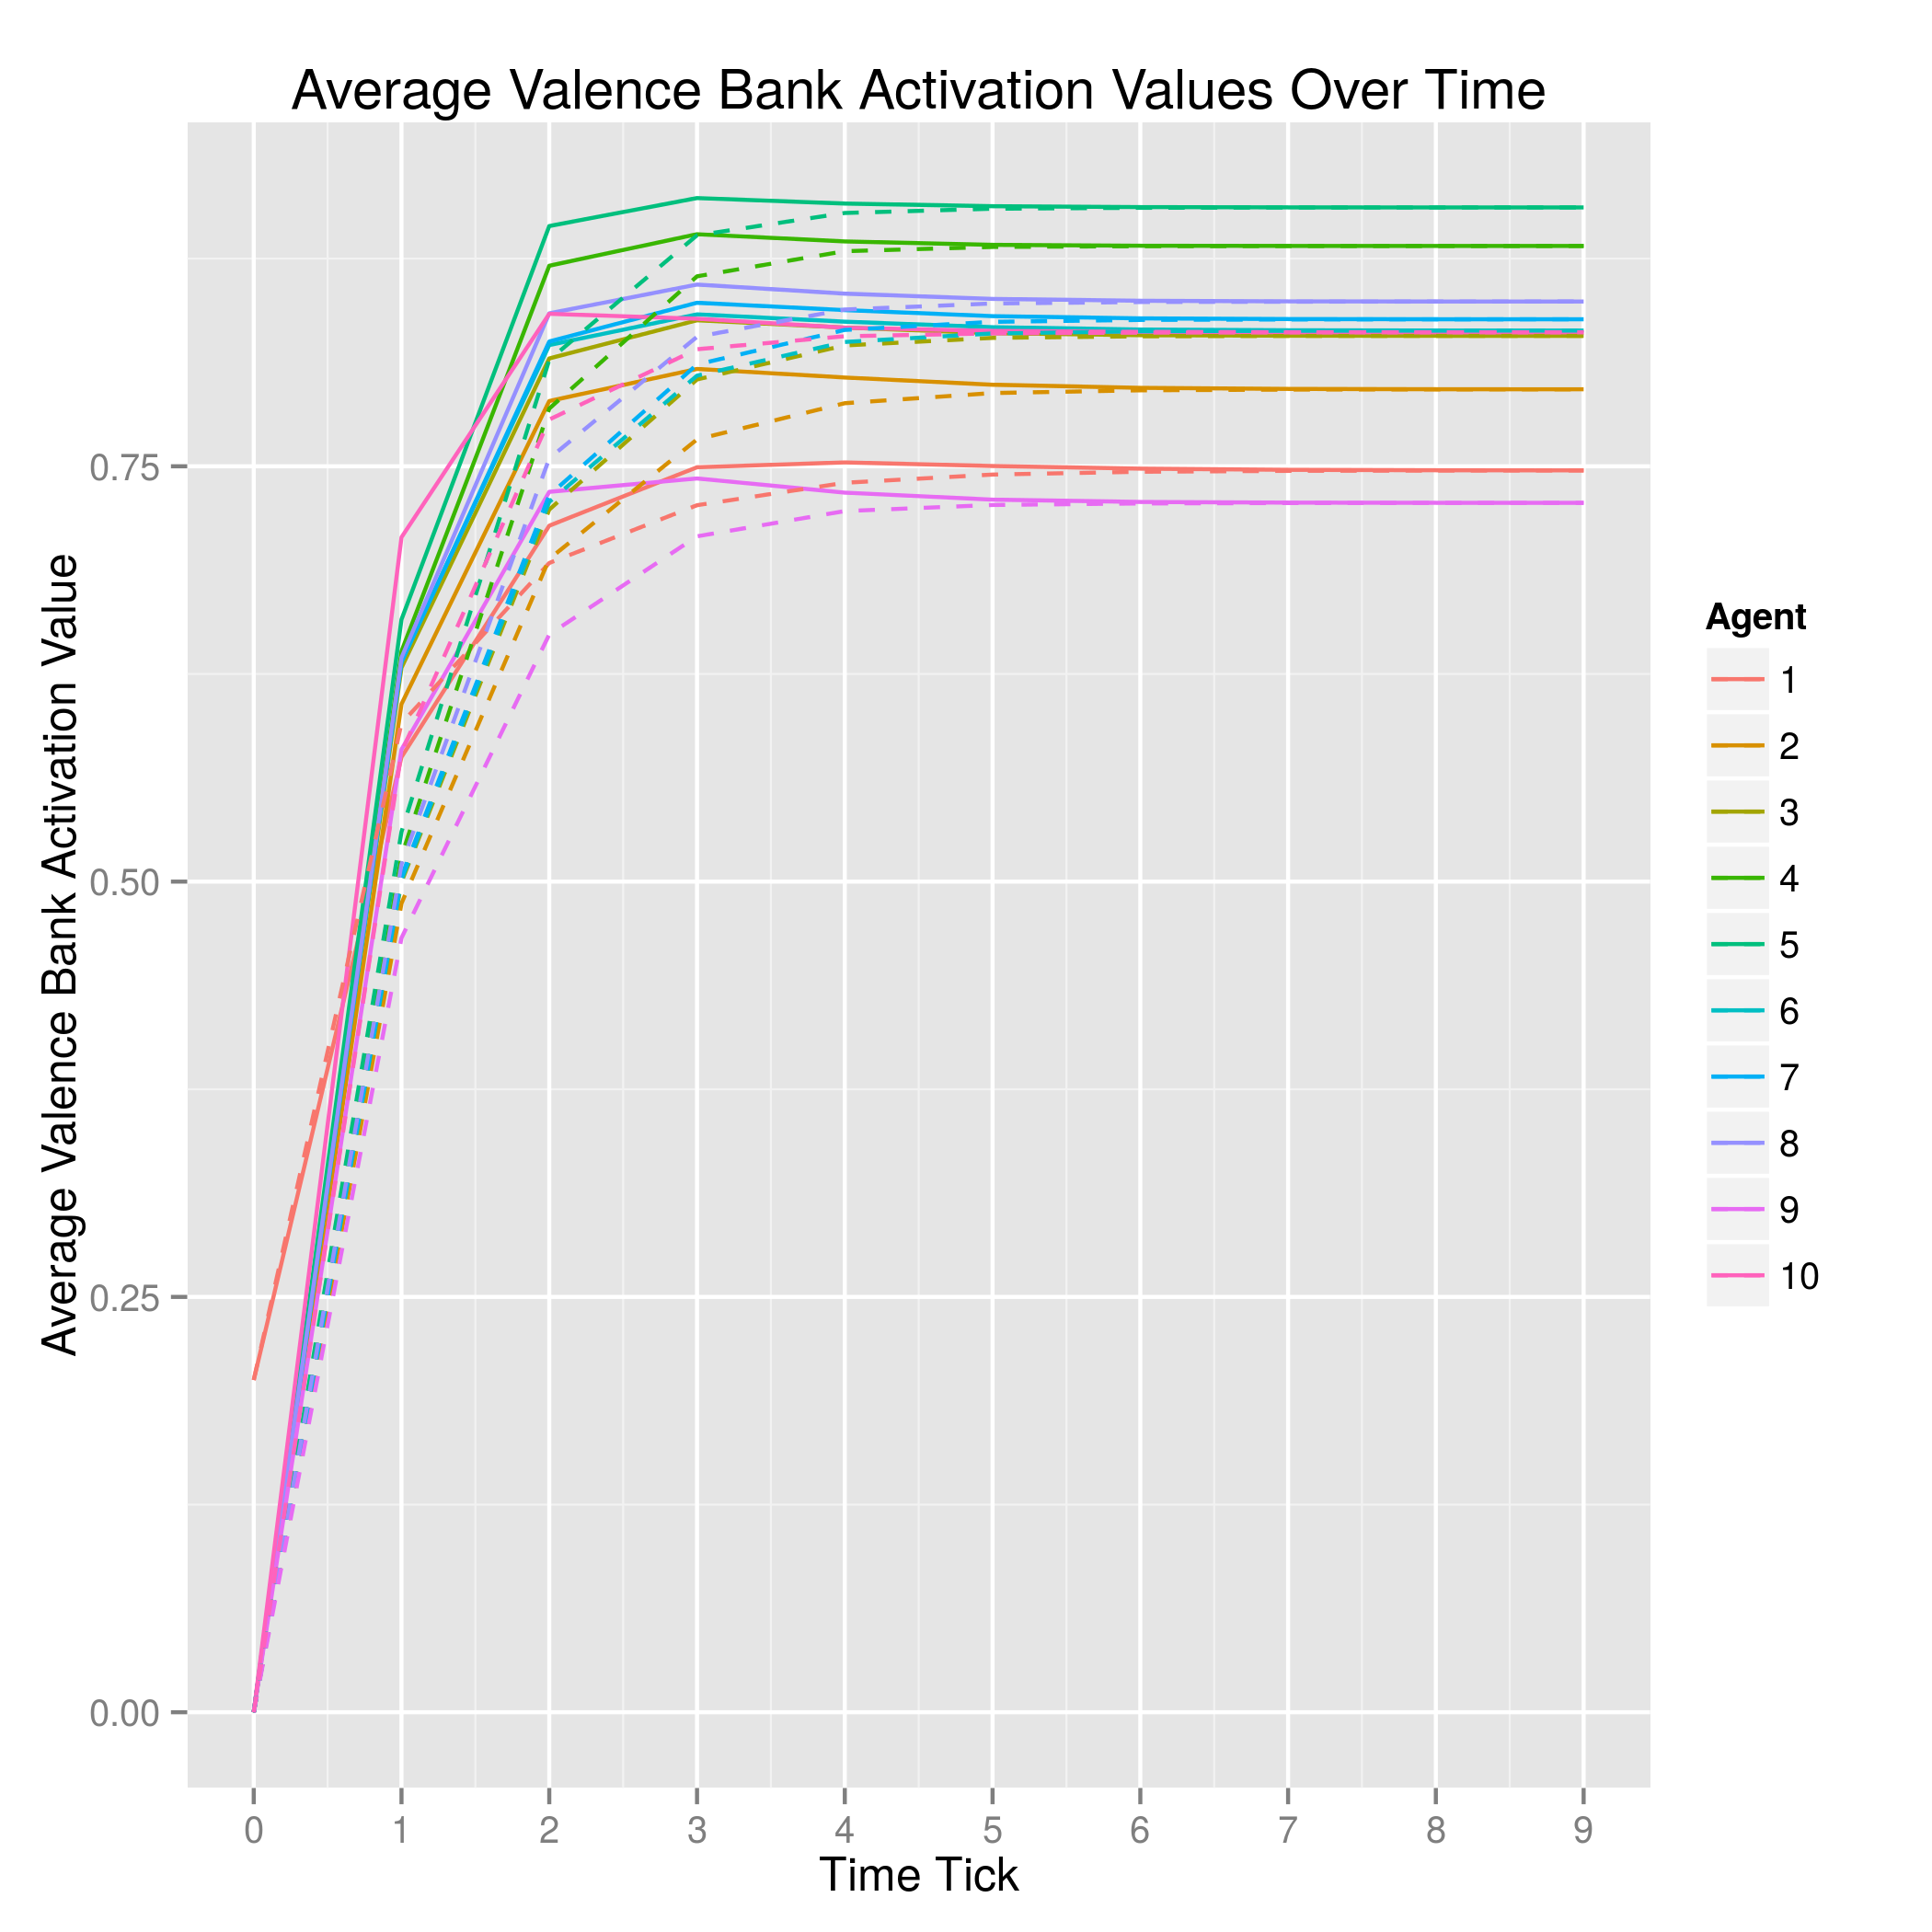
\includegraphics[width=\maxwidth]{figure/plot-sanity-8} \caption[Sanity Checking 8]{Sanity Checking 8\label{fig:plot-sanity-8}}
\end{figure}


\end{knitrout}


\newpage
\subsection{Sanity 9}
\label{sec:sanity9}
\begin{itemize}
  \item Agents Activated: \textbf{1}
  \item Valence Bank: both
  \begin{itemize}
      \item Valence bank activation: first positive, last negative
  \end{itemize}
  \item Valence bank Weights: random
  \begin{itemize}
      \item opposite -0.2
      \item corresponding 0.5
      \item carry over = \textbf{0.7}
      \item bias = 0
      \item decay = -0.5
  \end{itemize}
  \item Network: circle
\end{itemize}
\begin{knitrout}
\definecolor{shadecolor}{rgb}{0.969, 0.969, 0.969}\color{fgcolor}\begin{kframe}
\begin{alltt}
\hlkwd{plot.thesis.data}\hlstd{(}\hlstr{"../data/sanity/sanity9.csv"}\hlstd{,} \hlkwc{numAgents} \hlstd{=} \hlnum{10}\hlstd{,} \hlkwc{numTimeTicks} \hlstd{=} \hlnum{10}\hlstd{)}
\end{alltt}
\end{kframe}\begin{figure}[]

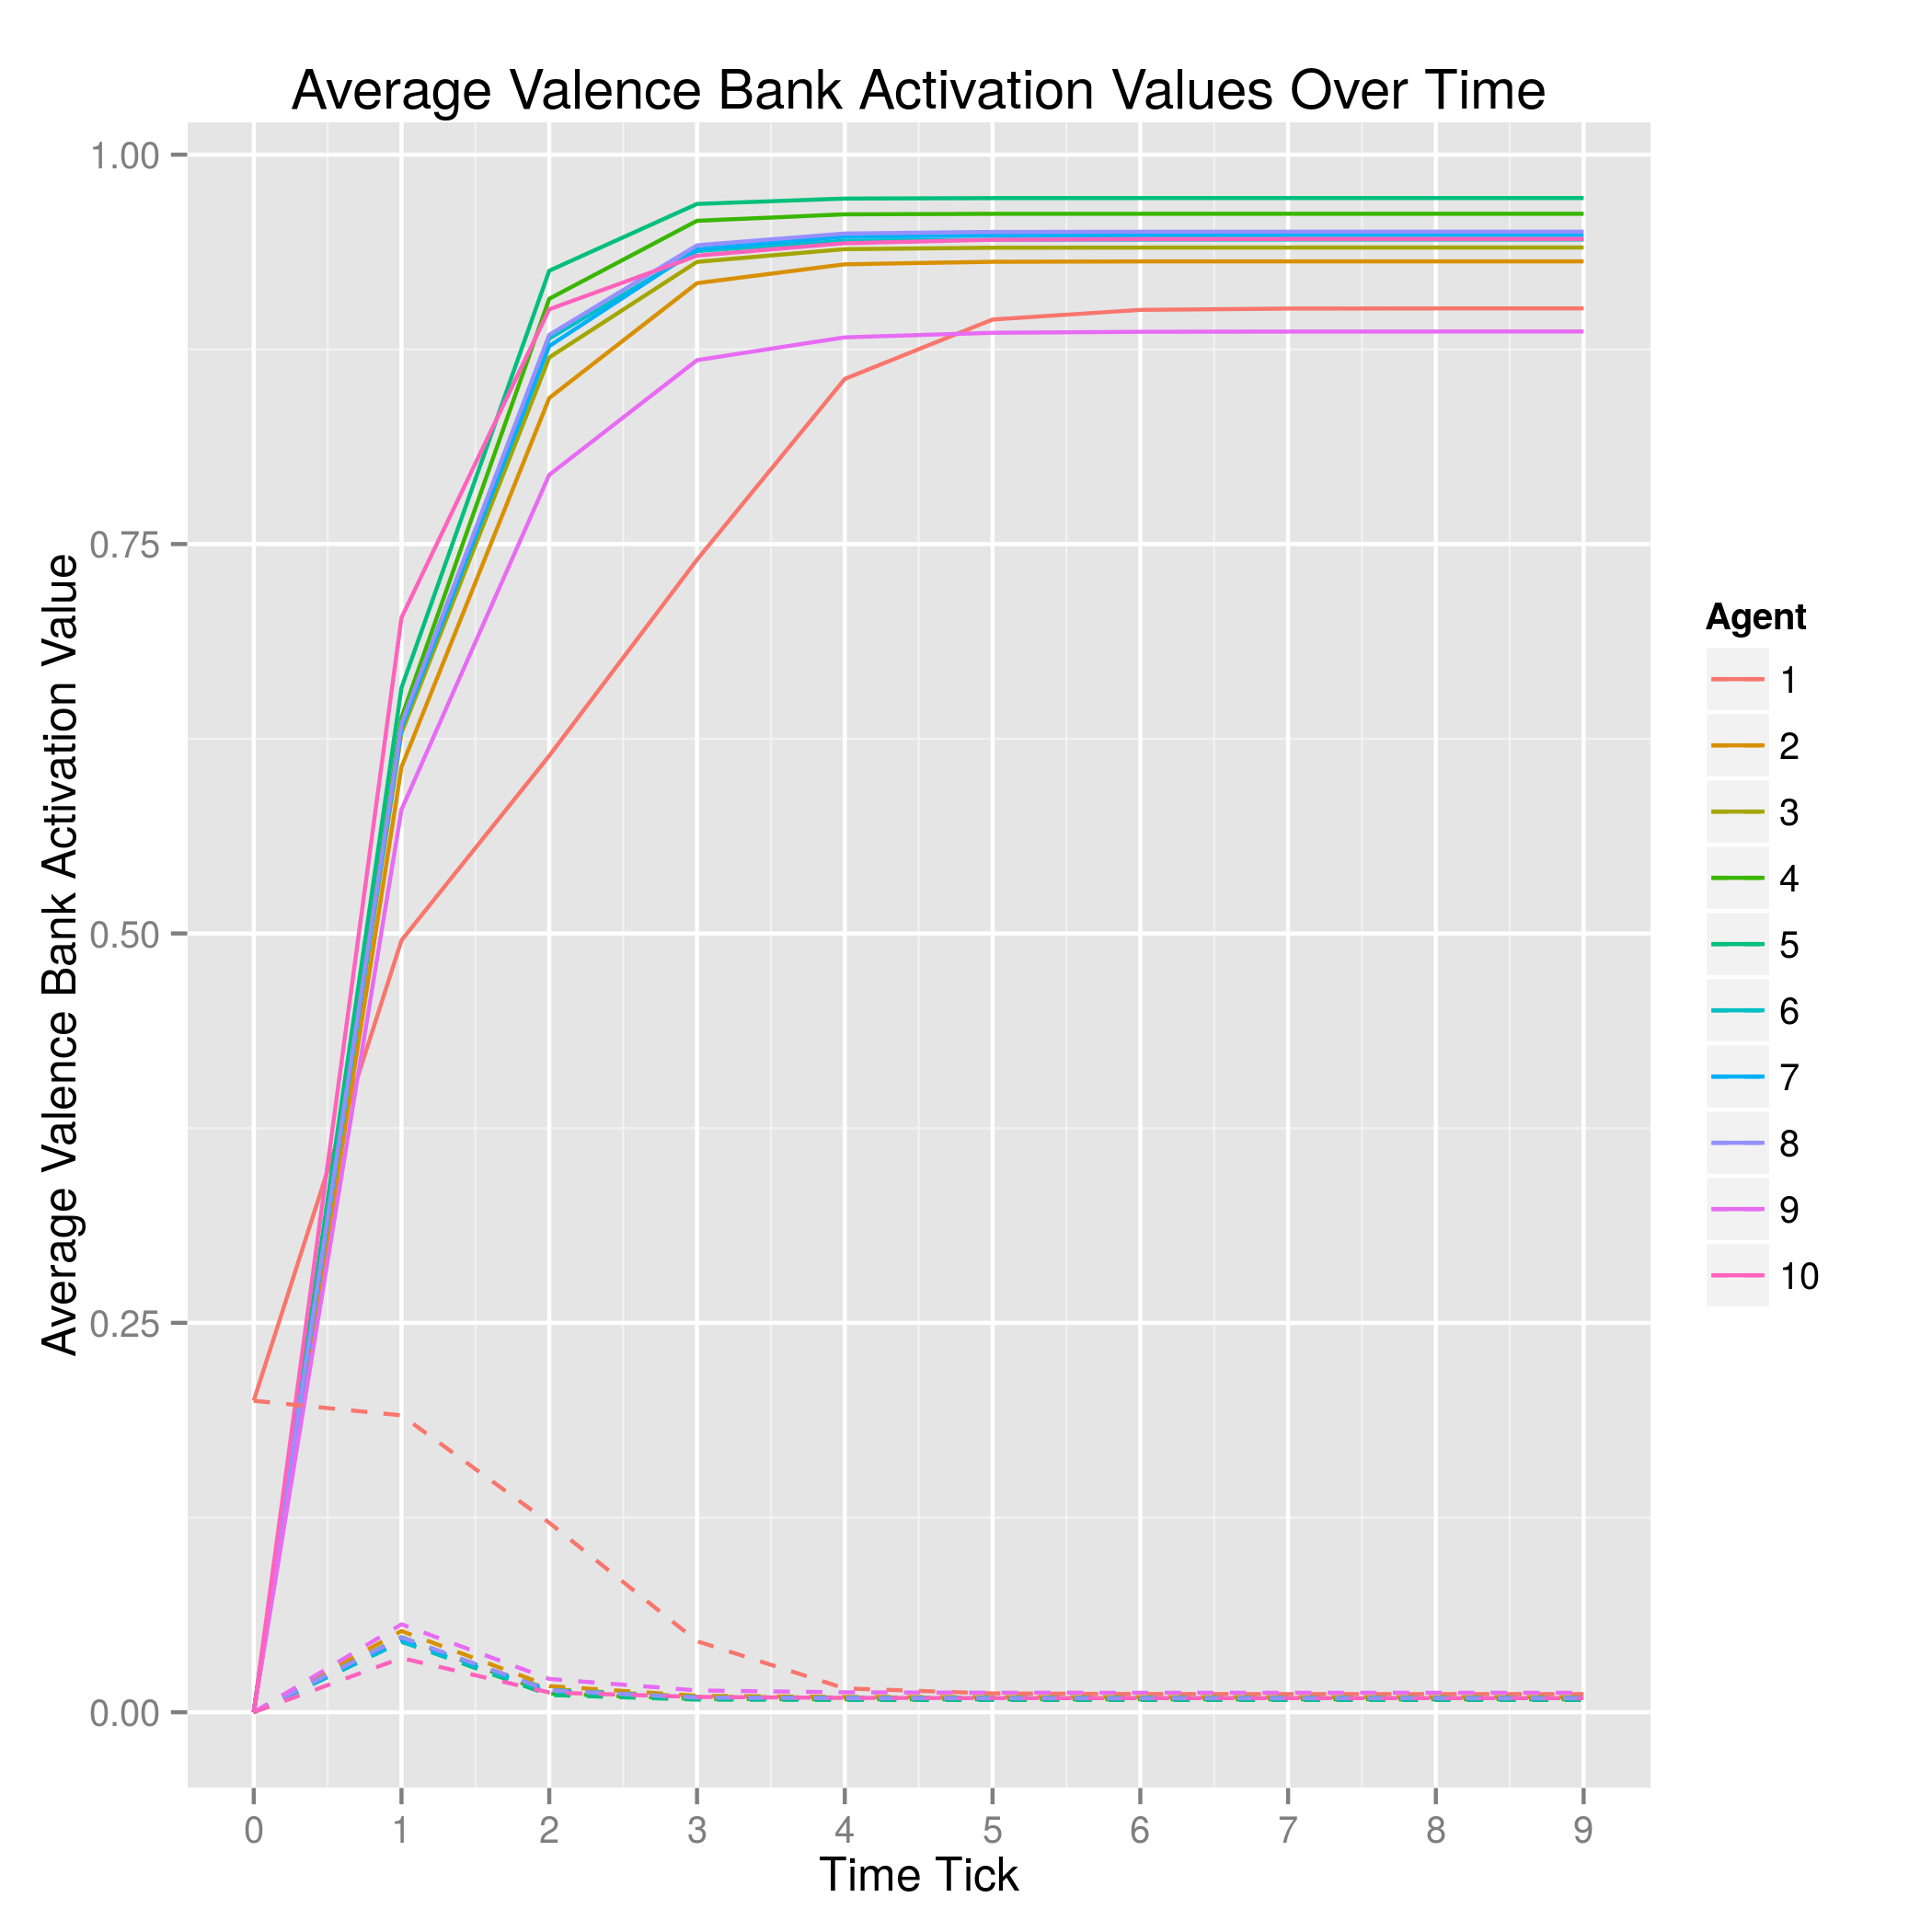
\includegraphics[width=\maxwidth]{figure/plot-sanity-9} \caption[Sanity Checking 9]{Sanity Checking 9\label{fig:plot-sanity-9}}
\end{figure}


\end{knitrout}

%
% \newpage
% \subsection{Sanity 10: 1-5}
% <<>>=
% plot.thesis.data("../data/sanity/sanity10-1.csv", numAgents=10, numTimeTicks=10)
% @
% \newpage
% <<>>=
% plot.thesis.data("../data/sanity/sanity10-2.csv", numAgents=10, numTimeTicks=10)
% @
% \newpage
% <<>>=
% plot.thesis.data("../data/sanity/sanity10-3.csv", numAgents=10, numTimeTicks=10)
% @
% \newpage
% <<>>=
% plot.thesis.data("../data/sanity/sanity10-4.csv", numAgents=10, numTimeTicks=10)
% @
% \newpage
% <<>>=
% plot.thesis.data("../data/sanity/sanity10-5.csv", numAgents=10, numTimeTicks=10)
% @
%
% \newpage
% \subsection{Sanity 11: 20 runs}
% <<>>=
% source(file = '../plot-function-ggplot2.R')
% plot.multiple.run.data("../data/sanity/sanity11.csv", numAgents=10, numTimeTicks=10)
% @

\end{document}
